\documentclass[11pt,oneside]{uhthesis}
%\documentclass[11pt,oneside]{report}
\usepackage{subfigure}
\usepackage[linesnumbered,lined,titlenumbered,ruled,algochapter,spanish,onelanguage]{algorithm2e}


\usepackage{substr}
\usepackage{bbm}
\usepackage{lipsum}
%\usepackage{easyReview}

\usepackage{amsmath}
\usepackage{theorem}
\usepackage{amssymb}
\usepackage{amsbsy}
%\usepackage{mathpazo}


\usepackage{float}
\usepackage{braket}
\usepackage[htt]{hyphenat}
\setlength {\marginparwidth }{3cm}


\usepackage[spanish]{babel}
\usepackage{graphicx}

\usepackage{listings}
\usepackage{color}
\usepackage{booktabs}
\usepackage{multirow}
\usepackage{ragged2e}
\usepackage{multicol}
\usepackage{comment} 

\usepackage{hyphenat}
\hyphenation{in-te-rac-tú-an}

\spanishdecimal{.}

\floatstyle{ruled}
\restylefloat{table}
\usepackage{color}

\usepackage[disable]{todonotes}

\definecolor{dkgreen}{rgb}{0,0.6,0}
\definecolor{gray}{rgb}{0.2,0,0}
\definecolor{mauve}{rgb}{0.58,0,0.82}

\lstset{language=Python,
	aboveskip=10mm,
	belowskip=10mm,
	showstringspaces=false,
	columns=flexible,
	basicstyle={\small\ttfamily},
	keywordstyle=\color{blue},
	commentstyle=\color{dkgreen},
	stringstyle=\color{mauve},
	breaklines=true,
	breakatwhitespace=true,
	tabsize=3,
	numbers=left, numberstyle=\tiny, stepnumber=1,firstnumber=1,
	numbersep=5pt
}

\renewcommand{\tablename}{Tabla}
\title{Simulador de sistema inmune para predecir la respuesta de lactantes a vacunas antineumocócicas conjugadas}
\author{Amanda Cordero Lezcano}
\advisor{MSc. Celia T. González González \\ MSc. Wilfredo Morales Lezca}
\degree{Licenciado en Ciencia de la Computación}
\faculty{Facultad de Matemática y Computación}
\date{Junio 2025}
\logo{Graphics/uhlogo}

\renewcommand{\vec}[1]{\boldsymbol{#1}}
\newcommand{\diff}[1]{\ensuremath{\mathrm{d}#1}}

% Comandos Lachi

% Para poner notas con autor Lachi
\newcommand{\lachinote}[2][noinline]{\todo[author=Lachi,backgroundcolor=cyan,linecolor=cyan,#1]{\footnotesize {#2}}}

\newcommand{\correccion}[2][noinline]{\todo[backgroundcolor=pink,linecolor=pink,#1]{\scriptsize {#2}}}



% Para definir teoremas, lemas, definiciones, corolarios, pruebas

\newtheorem{definicion}{Definición}
\newtheorem{lema}{Lema}
\theoremstyle{break}
\newtheorem{teorema}{Teorema}
\theoremstyle{break}
\newtheorem{corolario}{Corolario}[teorema]
\newtheorem{prueba}{Prueba}
%\theoremstyle{break}

% Para citar teoremas, lemas, definiciones, corolarios, pruebas
\newcommand{\reftheorem}[1]{\IfBeforeSubStringEmpty{teorema}{#1}{\textbf{Teorema~\ref{#1}}}{\IfBeforeSubStringEmpty{lema}{#1}{\textbf{Lema~\ref{#1}}}{\IfBeforeSubStringEmpty{prueba}{#1}{\textbf{Prueba~\ref{#1}}}{\IfBeforeSubStringEmpty{corolario}{#1}{\textbf{Corolario~\ref{#1}}}{\IfBeforeSubStringEmpty{definicion}{#1}{\textbf{Definición~\ref{#1}}}{{\color{red} Citado Erróneo}}}}}}}

\newcommand{\reftheorempage}[1]{\IfBeforeSubStringEmpty{teorema}{#1}{\textbf{Teorema~\ref{#1}} (pág \pageref{#1})}{\IfBeforeSubStringEmpty{lema}{#1}{\textbf{Lema~\ref{#1}} (pág \pageref{#1})}{\IfBeforeSubStringEmpty{prueba}{#1}{\textbf{Prueba~\ref{#1}} (pág \pageref{#1})}{\IfBeforeSubStringEmpty{corolario}{#1}{\textbf{Corolario~\ref{#1}} (pág \pageref{#1})}{\IfBeforeSubStringEmpty{definicion}{#1}{\textbf{Definición~ \ref{#1}} (pág \pageref{#1})}{{\color{red} Citado Erróneo}}}}}}}

\begin{document}
\selectlanguage{spanish}

%\frontmatter
\maketitle

\begin{dedication}
	\textit{“Todos los modelos son incorrectos, pero algunos son útiles”}
	
		George E. Pelham Box\\\vspace{0.7cm}
\end{dedication}
% \chapter*{Agradecimientos}\label{chapter:agradecimientos}

Pending...




\begin{opinion}	

	Pending...
\vspace{1cm}

\begin{flushleft}
	%\underline{\hspace{6.5cm}}\\
	% \qquad La Habana, 4 de enero de 2024.
	
	% \qquad DrC. José Alejandro Mesejo Chiong
	
	% \qquad DrC. Angela Mireya León Mecías
	
	% \qquad Facultad de Matemática y Computación
	
	% \qquad Universidad de la Habana
\end{flushleft}

\end{opinion}
\begin{abstract}
	Las enfermedades causadas por \textit{Streptococcus pneumoniae} representan un importante problema de salud pública, especialmente en lactantes. Este trabajo presenta el desarrollo de un simulador computacional del sistema inmune infantil para predecir la efectividad de la vacuna antineumocócica conjugada Quimi-Vio7\textregistered. El modelo implementado representa los componentes clave del sistema inmune, incluyendo células B, antígenos y la dinámica de los centros germinales. Se emplearon datos reales de ensayos clínicos con la vacuna VCN7-T para validar el modelo, utilizando la distancia de Chamfer como métrica de similitud entre los resultados simulados y los datos experimentales. 
	% Los resultados muestran que el simulador puede capturar adecuadamente la variabilidad en las respuestas inmunes para diferentes serotipos neumocócicos, con distancias de Chamfer que oscilan entre 2.773 (serotipo 18C) y 26.348 (serotipo 14). 
	Este enfoque computacional ofrece una herramienta para acelerar el desarrollo y evaluación de vacunas, reduciendo la dependencia de ensayos clínicos extensivos.

\end{abstract}

\begin{enabstract}
    Diseases caused by \textit{Streptococcus pneumoniae} represent a significant public health problem, particularly in infants. This work presents the development of a computational simulator of the infant immune system to predict the effectiveness of the pneumococcal conjugate vaccine Quimi-Vio7\textregistered. The implemented model represents key immune system components, including B cells, antigens, and germinal center dynamics. Real clinical trial data with the VCN7-T vaccine were used to validate the model, employing the Chamfer distance as a similarity metric between simulated results and experimental data. 
	% The results show that the simulator can adequately capture variability in immune responses for different pneumococcal serotypes, with Chamfer distances ranging from 2.773 (serotype 18C) to 26.348 (serotype 14).
	This computational approach offers a tool to accelerate vaccine development and evaluation, reducing dependence on extensive clinical trials.
\end{enabstract}
\tableofcontents
\listoffigures
\listoftables


%\mainmatter
	
%===================================================================================
% Chapter: Introduction
%===================================================================================
\chapter*{Introducción}\label{chapter:introduction}
\addcontentsline{toc}{chapter}{Introducción}
%===================================================================================

% Bacteriología y Virulencia
% Bacteria encapsulada: La cápsula de polisacárido es el principal factor de virulencia.
% Se han identificado más de 90 serotipos en el mundo, pero solo unos pocos causan la mayoría de las enfermedades en lactantes.
% Carga de la Enfermedad
% Transmisión: A través de secreciones respiratorias (pacientes o portadores).
% Infecciones graves: Neumonía, meningitis, bacteriemia.
% Infecciones comunes: Otitis media, sinusitis, bronquitis.


% Las enfermedades causadas por Streptococcus pneumoniae (el neumococo) son un importante problema de salud pública en todo el mundo. En los países en desarrollo, los niños pequeños y los ancianos son los más afectados; se estima que alrededor de un millón de niños mueren cada año a causa de enfermedades neumocócicas.

% Una vacuna desarrollada a partir de polisacáridos capsulares (PsC) de diferentes serotipos de Streptococcus pneumoniae, conjugados a una proteína portadora. Esta conjugación convierte
% la respuesta inmune inducida de T-independiente a T-dependiente, mejorando la inmunogenicidad y la protección a largo plazo.

% Las infecciones por Streptococcus pneumoniae son la primera causa de muerte por
% enfermedades inmunoprevenibles en los niños menores de 5 años y causan alrededor de un
% millón de fallecimientos anuales en la infancia, lo que representa la mitad de la mortalidad en
% todas las edades, de acuerdo con estimaciones de la Organización Mundial de la Salud (OMS)
% (1).
% Las neumonías, sepsis y meningitis comprenden más de 25\% de los 10 millones de estas
% muertes. La OMS estima que
% aproximadamente 1.6
% millones de muertes son causadas
% anualmente por esta bacteria. El 90\% de estas muertes ocurren en los países en vías de
% desarrollo y de ellas entre 700 000 a un millón se producen en niños menores de cinco años. El
% organismo internacional reconoce, además, que son afectados 14.5 millones niños menores de 5
% años con episodios graves de neumonía, de los cuales unos 8000 mueren, la mayoría de ellos en
% países de bajos y medios ingresos (1).
% La enfermedad neumocócica es el término que se utiliza para describir de forma general las
% infecciones causadas por la bacteria Streptococcus pneumoniae. Incluye la Enfermedad
% Neumocócica Invasiva (ENI) definida por el aislamiento del neumococo en fluidos corporales
% normalmente estériles, que produce meningitis, sepsis y neumonía bacteriémica y otras como la
% peritonitis, la artritis y la osteomielitis. La enfermedad tiene además otras formas no invasivas
% como son: las neumonías no bacteriémicas y otitis media. De todas las manifestaciones, las
% formas invasivas de la enfermedad están asociadas con alta tasa de mortalidad y elevados costos
% de hospitalización y tratamientos (2).

% En la actualidad se conocen más de 90 serotipos de neumococo, por lo que el enfrentamiento a
% este patógeno se torna más complejo que lo tradicionalmente establecido para las infecciones
% causadas por bacterias (5).

% Las enfermedades neumocócicas afectan principalmente a los niños más pequeños y los adultos
% mayores, siendo las neumonías, meningitis, otitis media, sinusitis y sepsis las formas más
% frecuentes de la enfermedad (9,10). La ENI tiene una mortalidad media de 10\%, que puede
% elevarse a más del 30\% en los grupos de riesgo (11). Además de la elevada mortalidad infantil
% por esta causa, el neumococo causa una carga estimada de 14,5 millones de episodios de
% enfermedad grave en niños pequeños cada año.
% La incidencia de la enfermedad neumocóccica depende de múltiples factores, como la edad, el
% área geográfica, las condiciones socioeconómicas y el estado de inmunocompetencia de los
% individuos (12,13). La existencia de más de 90 serotipos inmunológicamente distintos,
% determinados por la composición de la cápsula de polisacáridos, complica notablemente la
% descripción epidemiológica de este germen. Estudios epidemiológicos regionales que estiman la
% proporción de ENI en niños menores de 5 años, demuestran que un limitado número de
% serotipos causan la mayoría (más del 70\%) de las ENI a nivel mundial. Por ello, el número de
% serotipos fue determinado geográficamente y presenta la siguiente distribución por continentes: 6
% serotipos en América del Norte, 9 en África y 11 en Asia. Mundialmente, siete serotipos (1, 5, 6A,
% 6B, 14, 19F y 23F) fueron los más comunes asociados a la incidencia de ENI (14). Por ejemplo, el
% serotipo 14 fue el más común en todas las regiones del mundo, relacionado con el 12-29\% de
% todas las ENI. El serotipo 6A y 6B se ubicó en el segundo lugar en cada región, excepto en África
% con el 14-18\% de las ENI. Los serotipos 1, 5 y 14 estan presentes en el 28-43\% de las ENI a
% nivel mundial y son también los más comunes en muchos de los países de Latinoamérica (15),
% por eso la recomendación de la OMS de que estos tres serotipos deben estar incluidos en
% cualquier nueva vacuna contra los neumococos (16). En Cuba, la enfermedad neumocócica
% constituye actualmente la principal causa de
% enfermedad infecciosa bacteriana en niños
% pequeños, una vez introducidas en el país la vacunación contra el Haemophilus influenzae tipo B
% y Neisseria meningitidis serogrupo B y C. Sin embargo, los estudios epidemiológicos relacionados
% con los aislamientos de neumococo, realizados en Cuba en la última década son muy pobres. En
% el período 2000-2005 en el Instituto de Medicina Tropical “Pedro Kourí” de Cuba se realizaron un
% total de 1332 aislamientos (período con mayor número de aislamientos en los últimos 15 años).
% Los grupos más susceptibles resultaron ser los niños menores de 6 años con 842 casos y los
% adultos mayores de 60 años de edad con 302, y se concluyó que los serotipos aislados
% predominantes en el país son 1, 6B, 14, 18C, 19F, 23F con una alta susceptibilidad a las
% penicilinas y cefalosporinas (17). Otro estudio realizado recientemente por este Instituto evaluó
% el comportamiento de la meningitis bacteriana por Streptococcus pneumoniae en el período
% comprendido de Enero–Junio 2010. Se reportaron 34 casos, de los cuales en 19 se pudieron
% tipificar las cepas: 23F (21,5\%), 14 (21,5\%), 6A (0,38\%), 6B (0,38\%) y 4, 8, 17,15C, 18F, 19A y
% 23A (0,19\%). Se determinó que los serotipos 23F, 14, 6A y 6B continúan siendo los más
% frecuentes en el país (18).
% En el período 2007-2012 se reportaron 99 aislamientos en niños menores de 5 años, el número
% más bajo en todos estos años. A pesar de esta baja representatividad obtenida por estos
% aislamientos de lo que
% puede ser la circulación de la bacteria en el país, continúan siendo los serotipos 6B, 6A, 14 y 19F
% los más frecuentes, y se evidencia circulación del serotipo 19A (19,20)

% Desde inicios del siglo XX la comunidad científica demostró que los anticuerpos inducidos
% contra los polisacáridos de la cápsula del neumococo eran capaces de proteger a los individuos de
% las enfermedades causadas por estas bacterias. En 1977 se autorizó el uso de una vacuna de
% polisacáridos contra los 14 serotipos más prevalentes, la cual proporcionaba protección
% contra el 80% de cepas invasoras aisladas en Estados Unidos. En 1983 se le agregaron otros
% nueve serotipos para un total de 23, lo cual aumentó la protección contra más del 90% de las
% cepas aisladas en los países desarrollados. La vacuna de polisacáridos 23-valente contra el
% neumococo ha estado disponible por más de 25 años para su uso en individuos mayores de dos
% años de edad, con una buena efectividad en la prevención de la enfermedad neumocóccica en
% adultos y poblaciones de riesgo. Si bien los beneficios de la vacuna 23- valente son innegables,
% este tipo de vacunación tiene como limitación fundamental que no induce memoria inmunológica y
% no es efectiva en niños menores de 2 años (21,22).
% La necesidad de superar las limitaciones de la vacuna 23-valente condujo al desarrollo de
% nuevas vacunas conjugadas contra neumococos. Estas se basan en la conjugación covalente de
% los PsC a una proteína portadora, lo que induce una presentación más eficiente de los antígenos
% polisacarídicos al sistema inmune y son capaces de generar memoria inmunológica. Estas
% vacunas se desarrollan a partir de polisacáridos capsulares de diferentes serotipos de
% Streptococcus pneumoniae, conjugados con una proteína portadora, con el objetivo de transformar
% la respuesta inmune inducida de T-independiente a T- dependiente (23). El antecedente más
% exitoso de estas vacunas fue la vacuna conjugada contra Haemophilus influenzae tipo B (24,25).
% En el año 2000 se licenció la primera vacuna conjugada heptavalente contra el Streptococcus
% pneumoniae con el nombre comercial Prevnar 13®, desarrollada por la compañía farmacéutica
% Wyeth. La selección de los siete serotipos (4, 6B, 9V, 14, 18C, 19F y 23F) respondió a que estos
% fueron identificados como líderes, el 70 al 80 % aparecieron como causantes de la enfermedad
% invasora y resistencia a los antibióticos en los niños norteamericanos (26). Sin embargo, los datos
% epidemiológicos de los países Latinoamericanos y del Caribe demuestran claramente que los
% serotipos 1 y 5 son agentes importantes de la enfermedad invasora en toda la región y no están
% contenidos en esa formulación (17).
% Durante los años 2009-2010 se licenciaron otras dos vacunas conjugadas: Synflorix®, una vacuna
% decavalente de la compañía GSK, y Prevnar 13® de 13 valencias de la compañía Pfizer®.
% Las dos vacunas tomaron como referencia la original 7-valente, adicionándole 3 nuevos serotipos
% (1, 5 y 7F) y 6 nuevos serotipos (1, 3, 5, 7F, 6A y 19A) respectivamente (27,28).
% Las vacunas conjugadas antineumocócicas (PCV) han demostrado ser seguras y eficaces en
% niños menores de 5 años para prevenir tanto las formas invasivas como las no invasivas de la
% enfermedad neumocócica. La eficacia de Prevnar 13® 7 fue demostrada en la prevención del
% 97.4% de las ENI causadas por los serotipos vacunales (29), en una reducción de la mortalidad
% infantil en niños menores de 2 años y en un sustancial decrecimiento de las ENI en poblaciones
% no vacunadas (30,31).
% Teniendo en consideración la elevada carga de enfermedad neumocócica que ocurre en niños
% pequeños en todo el mundo, y la seguridad y eficacia de las vacunas conjugadas
% antineumocócicas, la OMS recomienda que debe ser una prioridad de los programas nacionales
% de inmunización la inclusión de esta vacunación, particularmente en países donde la
% mortalidad infantil en niños menores de 5 años es superior a 50/1000 nacidos vivos o donde
% más de 50000 niños mueren anualmente (32).
% Las actuales PCV han sido desarrolladas por compañías multinacionales y han estado
% disponibles por más de una década, con un indudable impacto en la salud. El elevado precio de
% estas vacunas ha imposibilitado la adquisición en muchos lugares del mundo, sin embargo, con
% esquemas especiales de financiamiento, se ha logrado llegar a un número muy elevado de
% países. No obstante, quedan muchos países y poblaciones que no han podido introducirla en sus
% esquemas de inmunización. Al cierre del año 2012, solo 86 (44%) de los 194 países miembros de
% la OMS han introducido la vacunación antineumocóccica en sus programas nacionales de
% vacunación, representando solo el 31% de todos los niños que nacen en el mundo (33).
% En el caso de Cuba, resulta estratégico lograr el desarrollo de nuestras propias vacunas para
% darle sostenibilidad al Programa de Inmunizaciones con el desarrollo de un fuerte Programa de
% Inmunizaciones.
% La OMS ha establecido correlatos de protección para las vacunas conjugadas contra neumococo,
% basados en estudios de eficacia clínica de la primera vacuna Prevnar 7 en lactantes. Estos
% correlatos se basan en la inducción de anticuerpos anti-PsC ≥0.35 µg/mL contra cada serotipo y
% títulos opsonofagocíticos superiores o iguales a 1:8. La demostración clínica de estos correlatos
% con criterio de no inferioridad respecto a vacuna comercial es un requisito exigido para el
% licenciamiento de nuevas vacunas antineumocócicas (34).

% El Programa Nacional de Inmunizaciones en Cuba es una de las fortalezas del Sistema Nacional
% de Salud (SNS), sustentado por la vacunación contra 13 enfermedades infecciosas bacterianas
% o virales con una alta producción de estas vacunas en el propio país. Sin embargo, no ha
% sido posible incluir en él, la vacunación antineumocóccica debido fundamentalmente al elevado
% costo de las vacunas comerciales. Basado en la exitosa experiencia del desarrollo e introducción
% en Cuba de una vacuna conjugada contra Haemophilus influenzae tipo B (39), el país decidió
% financiar un proyecto de investigación-desarrollo, con el objetivo de obtener una vacuna
% conjugada heptavalente contra los serotipos de mayor circulación en Cuba y en la región de
% las Américas. Soportado por las evidencias de circulación de neumococo que reportaban los
% estudios SIREVA, fundamentalmente en el quinquenio 2000-2005 (19), se decidió que el
% candidato vacunal cubano estaría compuesto por los serotipos 1, 5, 6B, 14, 18C, 19F y 23F, todos
% conjugados a la proteína portadora toxoide tetánico y adyuvado en fosfato de aluminio.
% A partir del año 2006, comenzó un intenso trabajo de investigación-desarrollo que resultó en el
% candidato vacunal objeto de la presente investigación clínica en lactantes, que es el final del
% desarrollo clínico.

% La estrategia desarrollada para la evaluación preclínica de VCN7-T se basó en la
% demostración de la inmunogenicidad y seguridad de la formulación, siguiendo las regulaciones
% nacionales e internacionales para la evaluación pre-clínica y toxicológica de vacunas (40). Los
% métodos serológicos para evaluar la inmunogenicidad de las vacunas conjugadas contra
% neumococo incluyen dos pruebas críticas: la cuantificación de IgG anti-PsC y la actividad
% opsonofagocítica de los anticuerpos inducidos por la vacunación. Adicionalmente, otras
% determinaciones como las clases y subclases de anticuerpos, la memoria inmunológica, la avidez
% y afinidad de los anticuerpos por el PsC complementan la información acerca de los mecanismos
% de respuesta inmune inducidos por la vacunación (41). Por tanto, la evaluación de la
% inmunogenicidad de VCN7-T fue enfocada fundamentalmente a la demostración de la inducción
% de anticuerpos opsonofagocíticos y patrones de respuesta inmune característicos de vacunas
% conjugadas. Durante la evaluación pre-clínica de la inmunogenicidad de la VCN7-T, se demostró
% en conejos y ratones la inducción de anticuerpos específicos por cada PsC con actividad
% opsonofagocítica contra la bacteria del serotipo correspondiente. Adicionalmente, se demostró en

% conejos la inducción de memoria inmunológica e inmunidad mucosal. En las evaluaciones pre-
% clínicas que se han realizado hasta el momento, la VCN7-T ha mostrado ser segura (41).
% El estudio de toxicidad aguda no mostró efectos en ratas Cenp: SPRD, culminando con una
% supervivencia del 100 %. No se observaron signos clínicos tóxicos. El comportamiento del peso
% corporal no mostró diferencias significativas entre grupos y sexos. No se produjeron variaciones
% en la temperatura rectal relacionadas con la administración de la vacuna. No se detectaron
% alteraciones anatomopatológicas sobre los órganos parenquimatosos (42). El estudio a dosis
% repetidas también demostró que la vacuna es segura, no causando alteraciones en el sitio de
% la administración propias del adyuvante de aluminio utilizado (43).
% Con el objetivo de evaluar la posible interferencia inmunológica del candidato vacunal cubano
% contra los neumococos, VCN7-T, con las vacunas Heberpenta-L (toxoides tetánico y diftérico,
% conjugado del polisacárido capsular de Haemophilus influenzae a toxoide tetánico, antígeno de
% superficie del virus de la hepatitis B y células completas de Bordetella pertussis) y VA-
% MENGOC-BC (vesículas de membrana externa del serogrupo B y polisacárido capsular del
% serogrupo C de Neisseria meningitidis), se diseñó un estudio experimental en conejos.
% Los resultados fueron los siguientes: no se observó interferencia de VCN7-T sobre la respuesta
% humoral contra toxoide diftérico y los antígenos meningocócicos (p>0.05). Para el caso de la
% respuesta humoral contra el oligosacárido de Haemophilus influenzae tipo B se observó una
% reducción
% estadísticamente
% no
% significativa
% (p>0.05).
% Adicionalmente,
% la
% administración
% concomitante de Heberpenta y VCN7-T, incrementaron dos veces los títulos de anticuerpos y la
% actividad protectora contra el toxoide tetánico, aunque no se encontraron diferencias
% estadísticamente significativas. Por último, la co-administración no indujo una reducción en el
% porciento de respondedores contra los polisacáridos neumocócicos contenidos en VCN7-T.
% En conclusión, la administración concomitante de VCN7-T, no indujo interferencias sobre los
% antígenos evaluados de Heberpenta-L y VA-MENGOC-BC. Además, no se observó interferencia
% de éstos sobre la respuesta inmune inducida por VCN7-T. Estos resultados preclínicos sugieren
% que VCN7-T, no debe resultar en un problema serio sobre la respuesta inmunitaria provocada por
% las vacunas licenciadas Heberpenta®-L y VA-MENGOC-BC, sin embargo, la interferencia clínica
% debe ser estudiada estrictamente durante los ensayos clínicos en lactantes (44).

% En el período 2012-2014 se diseñaron y ejecutaron 2 ensayos clínicos con el objetivo de
% demostrar la seguridad del candidato vacunal en diferentes grupos de edades.
% En el año 2012, concluyó un ensayo clínico Fase I en adultos entre 18 y 35 años, que tuvo como
% objetivo evaluar la seguridad de la VCN7-T y además explorar la inmunogenicidad de la misma.
% Consistió en un estudio monocéntrico, paralelo, controlado y aleatorizado. En este estudio VCN7-
% T demostró ser seguro, después de una dosis en este grupo etario. Los resultados de la
% evaluación de las variables concentración de anticuerpos y título opsonofagocítico, evidenciaron
% la capacidad de la vacuna VCN7-T de activar una respuesta inmune contra los antígenos que
% contiene (45).
% El otro ensayo clínico Fase I se realizó como un ensayo secuencial en niños de 4-5 años de
% edad (etapa 1) y lactantes de 7-8 meses (etapa 2). Los resultados de la etapa 1 demostraron que
% una dosis del candidato vacunal conjugado heptavalente contra neumococos en niños es segura,
% al no reportarse eventos adversos graves relacionados con su inmunización. En los sujetos
% inmunizados con VCN7-T, el comportamiento de los eventos adversos esperados locales fue de
% aparición en las primeras 72 horas posteriores a la inmunización y de una duración menor a los 3
% días. No se reportaron eventos adversos esperados locales severos. El dolor fue el evento
% adverso esperado de mayor incidencia. La incidencia de los eventos adversos esperados
% sistémicos fue baja, de aparición en las primeras 72 horas posteriores a la inmunización y de una
% duración menor a los 3 días. No se reportaron eventos adversos esperados sistémicos severos
% con relación de causalidad con la administración del producto. Los eventos adversos no
% esperados relacionados al uso de VCN7-T fueron: aumento de temperatura local, aumento de
% volumen en el sitio de puntura; todos con aparición y duración menor de 3 días post-vacunación.
% El perfil de seguridad mostrado por el candidato vacunal VCN7-T fue similar a la vacuna control
% Synflorix®. Aunque el tamaño de la muestra de este estudio fue muy pequeño, la exploración
% preliminar de la inmunogenicidad de este candidato vacunal en niños preescolares evidenció la
% capacidad de la vacuna VCN7-T de activar una respuesta inmune contra los antígenos que
% contiene en los niños vacunados. La variable del título Opsonofagocítico, demostró que para los
% serotipos 6B, 14, 18C, 19F y 23F el 100% de los sujetos tuvo valores ≥1:8, mientras que para los
% serotipos 1 y 5 entre el 60-70 % de los sujetos vacunados con la VCN7-T tuvieron valores ≥1:8,
% similar al resultado obtenido en los sujetos inmunizados con Synflorix®. El total de estos niños en
% la evaluación previa a la vacunación se encontraban desprotegidos mayoritariamente contra casi
% la totalidad de los serotipos vacunales. Para la variable Concentración de IgG, se demostró que
% todos los sujetos vacunados con VCN7-T incrementaron significativamente las concentraciones
% de IgG para los siete serotipos (46).


% En la etapa 2 de evaluación de la seguridad de VCN7-T en lactantes de 7-11 meses tampoco
% mostró eventos adversos graves inesperados. En los sujetos vacunados con VCN7-T, la aparición
% de los Eventos Adversos Esperados Locales fue en las primeras 72 horas posteriores a cada
% vacunación. La induración fue el evento adverso esperado más frecuente. Los Eventos
% Adversos
% Esperados
% Sistémicos
% se reportaron en las primeras 72 horas posteriores a la
% inmunización y tuvieron una duración menor a los 3 días. Los eventos adversos locales
% esperados se caracterizaron por presentar intensidades leves, moderadas y severas. La fiebre fue
% el Evento Adverso Sistémico Esperado más frecuente. En los sujetos inmunizados con VCN7-T
% no se reportaron Eventos
% Adversos
% No
% Esperados
% Severos
% que
% tuvieran relación de
% causalidad con la administración del producto. Un esquema 2p+1 del candidato vacunal
% conjugado heptavalente contra neumococos en lactantes de 7-8 meses de edad es seguro.
% Después de cumplimentar
% el
% esquema
% 2p+1,
% los
% lactantes
% que
% recibieron
% VCN7-T
% alcanzaron el 100% de seroprotección en 6 serotipos con respecto a la concentración de
% anticuerpos, el serotipo 5 alcanzó un 94.7%. Estos resultados fueron alcanzados después del
% análisis con los valores de corte de 0,20 µg/mL y 0,35 µg/mL. Igualmente, los lactantes que
% recibieron VCN7-T alcanzaron el 100% de seroprotección, según OPA para todos los serotipos
% (47).


Las enfermedades causadas por \textit{Streptococcus pneumoniae} constituyen un grave problema de salud pública a nivel mundial, siendo responsables de una significativa morbilidad y mortalidad, especialmente en las edades extremas de la vida, como niños y adultos mayores~\cite{WHO2019}. Este patógeno, grampositivo, encapsulado y con gran diversidad de serotipos, es el agente etiológico de infecciones como neumonía, meningitis y otitis media, y se le atribuye alrededor de un millón de defunciones anuales a nivel global~\cite{OBrien2009}. En Cuba, la vigilancia epidemiológica y el desarrollo de vacunas han sido esenciales para reducir la incidencia de estas enfermedades, aunque la variabilidad genética del neumococo y la aparición de cepas resistentes siguen representando desafíos importantes~\cite{Gonzalez2017}.

El desarrollo de vacunas antineumocócicas conjugadas ha sido un avance crucial en la prevención de estas infecciones, pero su diseño y evaluación requieren largos periodos de investigación y ensayos clínicos costosos, lo que retrasa la introducción de nuevas formulaciones y limita su impacto inmediato en la salud pública~\cite{Plotkin2017}. 

Diversos estudios han explorado los mecanismos inmunológicos involucrados en la defensa contra \textit{S. pneumoniae}, destacando el papel de la inmunidad innata y adaptativa. El reconocimiento inicial del patógeno es mediado por receptores de reconocimiento de patrón (PRRs), como los receptores tipo Toll y NOD, que desencadenan la activación de factores de transcripción y la producción de citoquinas inflamatorias, esenciales para la activación de la respuesta inmune específica~\cite{Janeway2002}. Sin embargo, la gran diversidad de serotipos, junto con los mecanismos de evasión bacteriana, hace que la predicción de la efectividad de las vacunas mediante métodos tradicionales sea un proceso lento y costoso.

El principal desafío actual es desarrollar herramientas innovadoras que permitan predecir la efectividad de nuevas vacunas antes de su aplicación masiva, optimizando así los recursos y acelerando el proceso de inmunización. En este contexto, la modelación computacional del sistema inmune surge como una alternativa prometedora~\cite{Castiglione2014}. Un simulador computacional puede modelar la interacción entre el sistema inmune humano y los diferentes serotipos de \textit{S. pneumoniae}, permitiendo obtener predicciones sobre la respuesta inmunológica sin depender exclusivamente de ensayos clínicos extensivos.

Los modelos matemáticos permiten representar y predecir situaciones epidémicas, estimar escenarios futuros y evaluar la efectividad de distintas estrategias de vacunación, facilitando la toma de decisiones en salud pública~\cite{SINC2021,UC3M2022}. Gracias a estos modelos, es posible simular la respuesta inmune a diferentes formulaciones vacunales, optimizar el diseño y desarrollo de nuevas vacunas. Además, la simulación computacional permite abordar la complejidad y no linealidad de las interacciones entre células y moléculas del sistema inmune, superando las limitaciones de los modelos tradicionales basados únicamente en ecuaciones diferenciales~\cite{UCI2007}. Herramientas avanzadas como los autómatas celulares, los sistemas basados en agentes y la inteligencia artificial están revolucionando el desarrollo vacunal, permitiendo la creación de vacunas más potentes y estables, así como la adaptación ágil a nuevas variantes y contextos epidemiológicos cambiantes~\cite{DW2023}. En consecuencia, la integración de la matemática y la computación en la investigación vacunal no solo contribuye al avance científico, sino que también agiliza y optimiza la respuesta frente a los desafíos actuales y futuros en la prevención de enfermedades inmunoprevenibles.

Quimi-Vio7® es una vacuna cubana desarrollada a partir de polisacáridos capsulares (PsC) de diferentes serotipos de Streptococcus pneumoniae, conjugados a una proteína portadora. 
% Esta conjugación convierte la respuesta inmune inducida de T-independiente a T-dependiente, mejorando la inmunogenicidad y la protección a largo plazo.
La misma se encuentra registrada para su uso en población preescolar. Sin embargo el ensayo clínico que demostraría su efectividad en lactantes fue interrumpido por la pandemia de la COVID-19.




\vspace{0.5cm}

El objetivo general de esta investigación es el desarrollo de un simulador computacional del sistema inmune de un lactante para la predicción de la efectividad de la vacuna Quimi-Vio7®.

Los objetivos específicos de esta investigación son:
\begin{itemize}
    \item Analizar los principales mecanismos inmunológicos involucrados en la respuesta a la vacuna antineumocócica conjugada.
    \item Diseñar y programar un modelo computacional que represente la interacción entre el sistema inmune y \textit{S. pneumoniae}.
    
    \item Comparar los resultadosdel simulador en diferentes esquemas de vacunación.
\end{itemize}

Este enfoque contribuye tanto al avance teórico en inmunología computacional como a la optimización práctica del proceso de desarrollo de vacunas de este tipo, con potencial para reducir costos y tiempos de investigación y mejorar la toma de decisiones en salud pública.

La hipótesis que guía esta investigación es que un simulador computacional del sistema inmune de un lactante puede predecir de manera confiable la efectividad de la vacuna Quimi-Vio7®, permitiendo optimizar el proceso de desarrollo y evaluación de vacunas antineumocócicas conjugadas en Cuba.

\vspace{0.5cm}

La tesis se estructura en seis capítulos:
\begin{enumerate}
    \item \textbf{Estado del Arte:} Analiza los antecedentes y actualidad en cuanto a la modelación de sistema inmune y su interacción con vacunas.
    \item \textbf{Marco teórico:} Aborda los fundamentos del sistema inmune, la biología de \textit{S. pneumoniae}, las vacunas conjugadas y los modelos computacionales existentes.
    
    \item \textbf{Metodología:} Describe el diseño y desarrollo del simulador, las fuentes de datos utilizadas y los criterios de validación empleados.
    \item \textbf{Resultados:} Expone y analiza los resultados obtenidos con el simulador.
    \item \textbf{Discusión:} Compara los resultados del simulador con datos reales, analiza sus limitaciones y discute su potencial de aplicación.
    \item \textbf{Conclusiones y recomendaciones:} Resume los principales hallazgos y plantea sugerencias para investigaciones futuras.
\end{enumerate}
 
%===================================================================================
% Chapter: Estado del Arte
%===================================================================================
\chapter{Estado del Arte}\label{chapter:estadoarte}
%\addcontentsline{toc}{chapter}{Estado del Arte}
%===================================================================================

Pending...


%===================================================================================
% Chapter: Marco Teorico
%===================================================================================
\chapter{Preliminares}\label{chapter:preliminares}
%\addcontentsline{toc}{chapter}{Marco Teórico}
%===================================================================================

En este capítulo se sientan las bases para el desarrollo de la investigación.

\section{Perspectiva Inmunológica}

\textit{Streptococcus pneumoniae} es una bacteria Gram-positiva, encapsulada y con forma lanceolada, que coloniza las vías respiratorias superiores en humanos. Es un patógeno de relevancia clínica global, asociado tanto a enfermedades invasivas (como meningitis, neumonía bacteriémica y sepsis) como a infecciones no invasivas (otitis media aguda y sinusitis) \cite{WHO2019}.



\subsection{Características clave}
\begin{itemize}
    \item \textbf{Variabilidad serotípica}: Existen más de 90 serotipos\footnote{Microorganismo infeccioso clasificado según los antígenos presentes en su superficie celular.} diferenciados por la composición de su cápsula polisacárida, aunque apenas 12 de ellos son responsables de mas del 80\% de las infecciones neumocóccicas invasoras \cite{PREADOJ2001}
    \item \textbf{Poblaciones vulnerables}: Lactantes, adultos mayores (mayores de 65 años) e individuos inmunocomprometidos presentan mayor riesgo de infección grave.
\end{itemize}

\subsubsection{Importancia de la vacunación}
La diversidad de serotipos y la emergencia de cepas resistentes a antibióticos subrayan la importancia de estrategias preventivas como la vacunación. Las vacunas conjugadas han demostrado reducir significativamente la incidencia de enfermedad neumocócica al inducir inmunidad específica frente a los serotipos más prevalentes \cite{Snedecor2020a}.

\subsection{Inmunología básica}

El sistema inmunitario humano responde a \textit{Streptococcus pneumoniae} mediante dos grandes componentes \cite{AEP2022}:

\begin{itemize}
    \item \textbf{Inmunidad innata}: Primera línea de defensa, compuesta por células como neutrófilos, macrófagos y células dendríticas, así como factores humorales como el sistema del complemento.
    \item \textbf{Inmunidad adaptativa}: Proporciona especificidad y memoria inmunológica, mediada por linfocitos T (CD4$^+$, CD8$^+$) y B.
\end{itemize}

\subsubsection{Respuesta inmune a \textit{Streptococcus pneumoniae}: linfocitos B, memoria inmunológica y anticuerpos}

Los linfocitos B son fundamentales en la defensa frente a \textit{Streptococcus pneumoniae}, especialmente tras la vacunación:
\begin{itemize}
    \item Producen anticuerpos específicos que neutralizan al patógeno.
    \item Experimentan maduración de afinidad y cambio de isotipo (por ejemplo, de IgM a IgG).
    \item Generan células de memoria que permiten una respuesta más rápida y eficaz ante exposiciones futuras.
\end{itemize}

\subsubsection{Características inmunológicas en lactantes}
\begin{itemize}
    \item \textbf{Anticuerpos maternos}: 
    \begin{itemize}
        \item Transferencia placentaria de IgG (especialmente IgG1) mediante el receptor FcRn.
        \item Protección adicional a través de IgA secretora en la leche materna.
        \item Posible \textit{blunting} (interferencia de anticuerpos maternos con la respuesta vacunal), aunque su impacto clínico es limitado.\cite{AEP2023Blunting}
    \end{itemize}
    \item \textbf{Desarrollo inmune}: El sistema inmunitario neonatal es funcional pero inmaduro, dependiendo inicialmente de la inmunidad materna.
\end{itemize}

\subsubsection{Definiciones clave}
\begin{itemize}
    \item \textbf{Inmunogenicidad}: Capacidad de una vacuna para inducir una respuesta inmunitaria medible (por ejemplo, producción de anticuerpos).
    \item \textbf{Efectividad clínica}: Protección real conferida contra la enfermedad en condiciones del mundo real.
    \item \textbf{Conjugación proteica}: Las vacunas conjugadas unen polisacáridos capsulares a proteínas transportadoras para potenciar la respuesta inmunitaria, especialmente en niños pequeños.
\end{itemize}

\subsection{Vacunas antineumocócicas conjugadas}


Las vacunas antineumocócicas conjugadas (PCV por sus siglas en inglés) emplean polisacáridos capsulares conjugados a proteínas para inducir una respuesta inmunitaria robusta y duradera y generar memoria inmunológica mediante la activación de linfocitos T y B.


\subsubsection{Cobertura y correlatos de protección}
Las formulaciones actuales de PCV cubren los serotipos más prevalentes y virulentos. Los correlatos de protección\footnote{Mediciones de parámetros inmunitarios que permiten predecir el grado de protección contra la infección o enfermedad inducida por un patógeno.} pueden variar según el serotipo y la vacuna específica, y son utilizados como criterios en ensayos clínicos y en la evaluación de programas de vacunación \cite{Snedecor2020a}.

\subsection{Examen ELISA}

El examen ELISA (Ensayo de Inmunoabsorción Ligado a Enzima) es una técnica inmunoenzimática ampliamente utilizada para la detección y cuantificación específica de antígenos o anticuerpos en muestras biológicas. El principio fundamental del ELISA se basa en la unión específica entre un anticuerpo y un antígeno, donde uno de estos componentes está inmovilizado en una superficie sólida, generalmente una placa de microtitulación.

La detección se realiza mediante un anticuerpo conjugado con una enzima, que al reaccionar con un sustrato específico produce un cambio de color proporcional a la cantidad de analito presente en la muestra. Este cambio es medido espectrofotométricamente, permitiendo cuantificar la concentración del antígeno o anticuerpo.

Existen diferentes formatos de ELISA, entre ellos:

\begin{itemize}
    \item \textbf{ELISA directo}: el anticuerpo marcado con enzima se une directamente al antígeno inmovilizado.
    \item \textbf{ELISA indirecto}: utiliza un anticuerpo primario para detectar el antígeno y un anticuerpo secundario marcado con enzima para amplificar la señal.
    \item \textbf{ELISA sándwich}: un anticuerpo captura el antígeno, y otro anticuerpo marcado con enzima detecta el antígeno capturado, aumentando la sensibilidad y especificidad.
    \item \textbf{ELISA competitivo}: el antígeno en la muestra compite con un antígeno marcado por la unión a un anticuerpo específico.
\end{itemize}

Esta técnica es fundamental en diagnóstico clínico, investigación biomédica y control de calidad, debido a su alta sensibilidad, especificidad y rapidez \cite{Lequin2005}.

\section{Perspectiva Matemático-Computacional}
En esta sección se analizan los conceptos teóricos sobre los que se fundamenta esta investigación. Temas como: Metaheurísticas, métricas de similitud y concurrencia serán tratados en las siguientes subsecciones.


\subsection{Metaheurísticas}
\label{sec:metaheuristicas}

Las metaheurísticas son estrategias de alto nivel diseñadas para encontrar soluciones aproximadas a problemas de optimización complejos, especialmente aquellos donde los métodos exactos son computacionalmente inviables. Estas técnicas, inspiradas frecuentemente en procesos naturales o comportamientos sociales, exploran espacios de soluciones de manera inteligente para escapar de óptimos locales y aproximarse al óptimo global \cite{Talbi2009}.

% \subsubsection{Características Fundamentales}
% Las metaheurísticas comparten propiedades clave que las distinguen de otros métodos de optimización:

% \begin{itemize}
%     \item \textbf{Alto nivel de abstracción}: Independientes del problema específico
%     \item \textbf{Tolerancia a la no linealidad}: Manejan funciones objetivo discontinuas o no diferenciables
%     \item \textbf{Exploración-estratificada}: Balance entre diversificación (exploración) e intensificación (explotación)
%     \item \textbf{Algoritmos no deterministas}: Incorporan elementos estocásticos
%     \item \textbf{Bajo requerimiento de información}: No necesitan gradientes ni propiedades matemáticas específicas
% \end{itemize}


A continuación se presentan algunas de las metaheurísticas más conocidas:

\subsubsection{Recocido Simulado (Simulated Annealing)}
\label{subsec:recocido-simulado}

Inspirado en el proceso metalúrgico de recocido, donde un material se calienta y luego se enfría gradualmente para reducir sus defectos \cite{Kirkpatrick1983}. Este método:

\begin{itemize}
    \item Comienza con una solución inicial $s_0$ y temperatura alta $T_0$
    \item En cada iteración, genera una solución vecina $s'$
    \item Acepta soluciones mejores ($f(s') < f(s)$) siempre
    \item Acepta soluciones peores con probabilidad $P = e^{-\Delta f / T}$ donde $\Delta f = f(s') - f(s)$
    \item Reduce temperatura gradualmente según esquema $T_{k+1} = \alpha T_k$ ($\alpha \in (0,1)$)
\end{itemize}

La curva de enfriamiento (disminución de $T$) controla el balance exploración-explotación:

\begin{equation}
T(k) = \frac{T_0}{\ln(1 + k)} \quad \text{(esquema logarítmico)}
\end{equation}



\subsubsection{Algoritmos Genéticos (Genetic Algorithms)}
\label{subsec:algoritmos-geneticos}

Basados en la evolución biológica mediante selección natural \cite{Holland1992}.

\begin{itemize}
    \item Representan soluciones como cromosomas (vectores)
    \item Operadores clave:
    \begin{itemize}
        \item \textbf{Selección}: Prefiere soluciones con mejor \textit{fitness}
        \item \textbf{Cruzamiento}: Combina partes de dos soluciones
        \item \textbf{Mutación}: Modifica aleatoriamente componentes
    \end{itemize}
    \item Mantienen una población de soluciones diversa
    \item Reemplazo generacional o estado estable
\end{itemize}

La aptitud (fitness) de una solución $s_i$ se calcula como:
\begin{equation}
fitness(s_i) = \frac{1}{1 + f(s_i)}
\end{equation}


\subsubsection{Optimización por Colonia de Hormigas (Ant Colony Optimization)}
\label{subsec:tabu-search}

La Optimización por Colonia de Hormigas es una metaheurística bioinspirada que emula el comportamiento colectivo de las hormigas reales en su búsqueda de caminos óptimos hacia fuentes de alimento. Cuando las hormigas exploran su entorno, depositan sustancias químicas llamadas feromonas que sirven como señalización para otras hormigas \cite{Dorigo1996}. Este mecanismo de comunicación indirecta (estigmergia) permite a la colonia encontrar rutas eficientes mediante:
\begin{itemize}
    
    \item Retroalimentación positiva: Caminos más cortos acumulan más feromonas al ser transitados más frecuentemente
    \item Evaporación dinámica: Las feromonas se evaporan gradualmente, evitando convergencia prematura
    \item Exploración estocástica: Decisiones basadas en probabilidades que balancean explotación y exploración
\end{itemize}

El proceso sigue estos pasos iterativos:

\begin{enumerate}
    \item \textit{Inicialización}: Feromonas uniformes en todos los caminos ($\tau_{ij} = \tau_0$)
    \item \textit{Construcción de soluciones}: Cada hormiga $k$ construye una solución completa mediante selección probabilística:
    \[
    p_{ij}^k = \frac{[\tau_{ij}]^\alpha \cdot [\eta_{ij}]^\beta}{\sum_{l \in N_i^k} [\tau_{il}]^\alpha \cdot [\eta_{il}]^\beta}
    \]
    donde $\eta_{ij}$ es información heurística (ej. $1/d_{ij}$)
    \item \textit{Actualización de feromonas}: Combinación de evaporación y depósito:
    \[
    \tau_{ij} \leftarrow (1 - \rho) \cdot \tau_{ij} + \sum_{k=1}^m \Delta \tau_{ij}^k
    \]
    \[
    \Delta \tau_{ij}^k = 
    \begin{cases} 
    Q/L_k & \text{si la hormiga } k \text{ usó } (i,j) \\
    0 & \text{otro caso}
    \end{cases}
    \]
    \item \textit{Reforzamiento elitista}: Las mejores soluciones históricas reciben depósito adicional
\end{enumerate}

\subsection{Métricas para comparar conjuntos (nubes) de puntos}


Para evaluar la similitud entre dos nubes de puntos, se utilizan diversas métricas según el contexto de análisis. A continuación se presentan los métodos más relevantes:

\subsubsection{Distancia Euclidiana Promedio}
\label{subsec:dist-euclid}
Mide la proximidad espacial absoluta entre puntos correspondientes:
\begin{equation}
D_{\text{avg}} = \frac{1}{n} \sum_{i=1}^n \sqrt{(x_i - x'_i)^2 + (y_i - y'_i)^2}
\end{equation}

\textbf{Características:}
\begin{itemize}
    \item Interpretación física directa (unidades espaciales)
    \item Sensible a traslaciones globales
    \item Cálculo computacionalmente eficiente $O(n)$
\end{itemize}

\subsubsection{Similitud del Coseno}
\label{subsec:cos-sim}
Evalúa la orientación relativa de los vectores posición, independiente de su magnitud:
\begin{equation}
S_{\cos} = \frac{\sum_{i=1}^n (x_i x'_i + y_i y'_i)}{\sqrt{\sum_{i=1}^n (x_i^2 + y_i^2)} \cdot \sqrt{\sum_{i=1}^n ({x'_i}^2 + {y'_i}^2)}}
\end{equation}

\textbf{Aplicaciones:}
\begin{itemize}
    \item Comparación de formas geométricas
    \item Análisis donde la posición absoluta es irrelevante
    \item Sistemas de coordenadas relativas
\end{itemize}

\subsubsection{Métrica Basada en Trabajo de Transformación}
\label{subsec:work-metric}
Calcula la energía requerida para transformar una nube en otra:
\begin{equation}
S_{\%} = 100 \cdot \left(1 - \frac{W}{W_{\max}}\right)
\end{equation}
donde $W$ es el trabajo computado y $W_{\max}$ el trabajo máximo teórico.

\textbf{Implementación:}
\begin{enumerate}
    \item Calcular la transformación óptima (traslación, rotación)
    \item Integrar las diferencias posicionales residuales
    \item Normalizar respecto a la peor transformación posible
\end{enumerate}


\subsubsection{Métricas de Clustering}
\label{subsec:cluster-metrics}
Evalúan relaciones intra e inter-conjuntos:
\begin{align}
D_{\text{intra}}^A &= \frac{1}{n(n-1)} \sum_{i \neq j} \|p_i^A - p_j^A\| \\
D_{\text{inter}}^{\min} &= \min_{i,j} \|p_i^A - p_j^B\| \\
H_{\text{hausdorff}} &= \max\left( \sup_{a \in A} \inf_{b \in B} \|a-b\|, \sup_{b \in B} \inf_{a \in A} \|a-b\| \right)
\end{align}

\textbf{Interpretación:}
\begin{itemize}
    \item $D_{\text{intra}}$: Compacidad de cada nube
    \item $D_{\text{inter}}^{\min}$: Proximidad mínima entre nubes
    \item $H_{\text{hausdorff}}$: Máxima discrepancia entre fronteras
\end{itemize}

\subsubsection{Distancia Chamfer}
Cuantifica la similitud entre dos conjuntos de puntos en el espacio. Evalúa la proximidad bidireccional entre cada punto de un conjunto y su vecino más cercano en el otro conjunto.

El cálculo de la distancia de Chamfer se realiza en dos pasos principales:

\begin{enumerate}
    \item Para cada punto en el primer conjunto, se encuentra el punto más cercano en el segundo conjunto y se calcula la distancia euclidiana entre ellos. Se obtiene el promedio de estas distancias.
    \item Se repite el procedimiento invirtiendo los roles de los conjuntos, es decir, desde el segundo conjunto hacia el primero.
\end{enumerate}

Se define como la suma (o promedio) de estos dos valores, formalmente expresada como:
\[
D_{\mathrm{Chamfer}}(S_1, S_2) = \frac{1}{|S_1|} \sum_{x \in S_1} \min_{y \in S_2} \|x - y\|_2 \;+\; \frac{1}{|S_2|} \sum_{y \in S_2} \min_{x \in S_1} \|y - x\|_2
\]
donde \(\|\cdot\|_2\) denota la distancia euclidiana.

Esta métrica es relevante porque permite evaluar de forma robusta la similitud entre nubes de puntos, incluso cuando los estos no están emparejados uno a uno. 

\subsection{Acercamiento a la concurrencia}
La programación concurrente es un paradigma esencial para maximizar la eficiencia en sistemas modernos, permitiendo la ejecución aparentemente simultánea de múltiples tareas. Su dominio es crucial para desarrollar aplicaciones escalables y receptivas, aunque introduce complejidades que requieren técnicas especializadas para garantizar la corrección y estabilidad del software. Los contenido tratados en lo adelante están fundamentados en lo tratado en \cite{tanenbaum2008modern}.

\subsubsection{Concurrencia vs. Paralelismo}
La concurrencia y el paralelismo son conceptos fundamentales en la programación moderna, aunque a menudo se confunden debido a su estrecha relación. La concurrencia se refiere a la capacidad de gestionar múltiples tareas de forma que parezcan avanzar al mismo tiempo, aunque no necesariamente se ejecuten simultáneamente. Esto se logra mediante la planificación eficiente del procesador, donde un único núcleo puede alternar entre diferentes tareas en intervalos de tiempo muy pequeños, creando la ilusión de ejecución simultánea. La concurrencia permite que varias tareas progresen de manera ordenada incluso cuando compiten por recursos limitados.

Por otro lado, el paralelismo implica la ejecución real y simultánea de múltiples tareas utilizando recursos físicos separados, como varios núcleos de CPU o dispositivos de cómputo dedicados. Su enfoque está orientado a acelerar procesos computacionalmente intensivos dividiendo el trabajo en partes que pueden resolverse en paralelo. Aunque todo paralelismo implica concurrencia, ya que las tareas deben coordinarse, no toda concurrencia requiere paralelismo. Esta distinción es crucial a la hora de diseñar sistemas que prioricen el rendimiento o la interacción con el usuario.

\subsubsection{Hilos}
Un hilo (\textit{thread}) es la unidad básica de ejecución dentro de un proceso, gestionada directamente por el sistema operativo. Los hilos permiten dividir un programa en componentes que pueden ejecutarse concurrentemente, lo que resulta especialmente útil para tareas que requieren manejo simultáneo de distintas operaciones. Una característica clave de los hilos es que comparten el espacio de memoria y los recursos del proceso padre, lo cual facilita la comunicación entre ellos, pero también introduce desafíos relacionados con la consistencia de datos.



\subsubsection{Retos en Programación Concurrente}
La programación concurrente presenta una serie de desafíos, siendo uno de los más comunes la condición de carrera (\textit{race condition}). Este fenómeno ocurre cuando dos o más hilos intentan acceder y modificar un recurso compartido simultáneamente, causando resultados inconsistentes o impredecibles. Para evitar este tipo de problemas, se utiliza la exclusión mutua, que garantiza que solo un hilo pueda acceder a un recurso crítico en un momento dado.

Entre las herramientas más utilizadas para implementar exclusión mutua están los semáforos, \textit{mutex} y monitores. Estas estructuras permiten controlar el acceso a secciones críticas del código y asegurar la integridad de los datos compartidos. 
Sin embargo, su uso incorrecto puede llevar a otro problema conocido como interbloqueo (\textit{deadlock}), que sucede cuando dos o más hilos quedan esperando indefinidamente por recursos que nunca serán liberados porque cada uno posee un recurso que el otro necesita. 
% \subsection{Conceptos Fundamentales de Concurrencia}
% \label{sec:fundamentos-concurrencia}

% \subsubsection{Concurrencia y Paralelismo}
% La \textbf{concurrencia} es la capacidad de un sistema para gestionar múltiples tareas \textit{aparentemente} simultáneas, mientras que el \textbf{paralelismo} implica la ejecución \textit{real simultánea} de tareas. Matemáticamente, para $n$ tareas:

% \begin{equation}
% \text{Concurrencia} \subseteq \{ \text{Interleaving} \cup \text{Paralelismo} \}
% \end{equation}

% El paralelismo requiere múltiples unidades de procesamiento (e.g., núcleos de CPU), mientras que la concurrencia puede lograrse en un solo núcleo mediante planificación.

% \subsubsection{Hilos (Threads)}
% Los \textbf{hilos} son la unidad básica de ejecución dentro de un proceso. Comparten memoria pero tienen stacks propios. Un conjunto de hilos se define como:

% \begin{lstlisting}[language=C++,caption=Creación de hilos en C++]
% #include <thread>
% void tarea() { /* ... */ }

% int main() {
%     std::thread hilo1(tarea);  // Hilo secundario
%     std::thread hilo2(tarea);
    
%     hilo1.join();  // Sincronización
%     hilo2.join();
% }
% \end{lstlisting}

% \subsubsection{Condición de Carrera (Race Condition)}
% Ocurre cuando múltiples hilos acceden concurrentemente a recursos compartidos \textbf{sin sincronización}, y el resultado depende del orden de ejecución. Formalmente:

% \[
% \text{Race Condition} \iff \exists \, r_i, r_j \in \text{Accesos} \mid (r_i \parallel r_j) \land \neg \text{Ordenado}
% \]

% \subsubsection{Sección Crítica}
% Segmento de código donde se accede a recursos compartidos que deben protegerse. Debe satisfacer tres propiedades:
% \begin{enumerate}
%     \item \textbf{Exclusión mutua}: Solo un hilo puede ejecutarla
%     \item \textbf{Progreso}: Si no hay hilos en SC, algún hilo puede entrar
%     \item \textbf{Espera acotada}: Número máximo de espera es finito
% \end{enumerate}

% \subsubsection{Exclusión Mutua}
% Mecanismo para garantizar que solo un hilo acceda a la sección crítica. Implementaciones comunes:

% \begin{itemize}
%     \item \textbf{Mutex}: Bloqueo binario
%     \begin{lstlisting}[language=Python]
% import threading
% mutex = threading.Lock()

% mutex.acquire()
% # Sección crítica
% mutex.release()
%     \end{lstlisting}
    
%     \item \textbf{Semáforos}: Contador para $n$ accesos
%     \item \textbf{Monitores}: Abstracción de alto nivel
% \end{itemize}

% \subsubsection{Interbloqueo (Deadlock)}
% Situación donde múltiples procesos/hilos se bloquean mutuamente esperando recursos. Requiere cuatro condiciones (Coffman):
% \begin{enumerate}
%     \item \textbf{Exclusión mutua}: Recurso no compartible
%     \item \textbf{Retención y espera}: Mantener recursos mientras se esperan otros
%     \item \textbf{No expropiación}: Los recursos no pueden ser forzosamente liberados
%     \item \textbf{Espera circular}: Ciclo de dependencias
% \end{enumerate}

% El deadlock puede modelarse como grafo dirigido donde $P \to R$ indica que proceso $P$ solicita recurso $R$, y $R \to P$ indica que $R$ está asignado a $P$. Un ciclo implica deadlock.

% \subsubsection{Técnicas de Prevención}
% \begin{table}[h]
% \centering
% \begin{tabular}{|l|c|c|}
% \hline
% \textbf{Técnica} & \textbf{Ventajas} & \textbf{Desventajas} \\ \hline
% Evitar espera circular & Sin deadlock & Baja utilización recursos \\ \hline
% Expropiación & Flexibilidad & Complejidad implementación \\ \hline
% Espera acotada & Determinismo & Difícil estimación \\ \hline
% \end{tabular}
% \caption{Comparación de técnicas anti-deadlock}
% \end{table}
% \end{section}

% \section{Paralelismo y Concurrencia en Sistemas Distribuidos}
% \label{sec:paralelismo}

% La computación moderna requiere el manejo eficiente de operaciones simultáneas, lo que ha impulsado el desarrollo de técnicas de paralelismo y concurrencia. Estas permiten ejecutar múltiples tareas de forma coordinada, optimizando el uso de recursos computacionales.

% \subsection{Conceptos Fundamentales}
% \begin{itemize}
%     \item \textbf{Paralelismo}: Ejecución simultánea de tareas en múltiples procesadores o núcleos.
%     \item \textbf{Concurrencia}: Capacidad de gestionar múltiples tareas que progresan solapadamente en el tiempo.
%     \item \textbf{Hilos}: Unidad básica de ejecución dentro de un proceso que comparte espacio de memoria.
% \end{itemize}

% \subsection{Retos en Programación Concurrente}
% \label{subsec:retos}

% \subsubsection{Condiciones de Carrera}
% Ocurren cuando múltiples hilos acceden concurrentemente a recursos compartidos sin sincronización adecuada, llevando a resultados impredecibles. Por ejemplo:

% \begin{lstlisting}[language=C,caption=Ejemplo de condición de carrera]
% int contador = 0;

% void* incrementar() {
%     for(int i=0; i<1000; i++){
%         contador++; // Operación no atómica
%     }
% }
% \end{lstlisting}

% \subsubsection{Secciones Críticas}
% Regiones de código que acceden a recursos compartidos y requieren ejecución atómica. Su manejo inadecuado puede generar:

% \begin{itemize}
%     \item \textbf{Interbloqueo}: Situación donde dos o más procesos se bloquean mutuamente esperando recursos.
%     \item \textbf{Inanición}: Imposibilidad de un proceso para acceder a recursos necesarios.
% \end{itemize}

% \subsection{Exclusión Mutua}
% \label{subsec:exclusion}

% Mecanismo fundamental para garantizar que solo un hilo acceda a una sección crítica simultáneamente. Debe cumplir cuatro propiedades esenciales:

% \begin{enumerate}
%     \item Exclusión mutua: Máximo un hilo en la sección crítica
%     \item Progreso: Decisión de entrada en tiempo finito
%     \item Espera limitada: Cota máxima de espera para cualquier hilo
%     \item Neutralidad: No asumir velocidades de procesador
% \end{enumerate}

% \subsubsection{Técnicas de Implementación}
% \begin{table}[h]
% \centering
% \caption{Comparación de métodos de exclusión mutua}
% \begin{tabular}{|l|c|c|}
% \hline
% \textbf{Método} & \textbf{Ventajas} & \textbf{Limitaciones} \\ \hline
% Semáforos & Sincronización flexible & Complejidad de uso \\ \hline
% Monitores & Encapsulación natural & Soporte lenguaje requerido \\ \hline
% Mutex & Bajo overhead & Solo exclusión binaria \\ \hline
% \end{tabular}
% \end{table}

% \subsubsection{Algoritmos Clásicos}
% \begin{itemize}
%     \item Algoritmo de Peterson (solución software para dos procesos)
%     \item Semáforos de Dijkstra (sincronización generalizada)
%     \item Cerrojos adaptativos (spinlocks + bloqueo kernel)
% \end{itemize}

% \subsection{Consideraciones de Diseño}
% La gestión efectiva de la concurrencia requiere:
% \begin{itemize}
%     \item Análisis de granularidad de bloqueos
%     \item Patrones de diseño como productor-consumidor
%     \item Detección temprana de interbloqueos mediante grafos de asignación
%     \item Uso de herramientas de análisis estático (ej. ThreadSanitizer)
% \end{itemize}

% Este conjunto de técnicas y consideraciones constituye la base para construir sistemas concurrentes robustos y eficientes, particularmente relevantes en entornos distribuidos y de alto rendimiento.

%===================================================================================
% Chapter: Metodologia
%===================================================================================
\chapter{Metodología}\label{chapter:metodologia}
%\addcontentsline{toc}{chapter}{Marco Teórico}
%===================================================================================

En este capítulo se describe la metodología y la estructura empleada en la implementación de un simulador computacional del sistema inmune de un lactante para modelar la respuesta a vacunas conjugadas neumocócicas.

El simulador se estructura en dos capas principales:
\begin{enumerate}
    \item Modelado de agentes biológicos:
        \begin{enumerate}
            \item Antígenos
            \item Células B
        \end{enumerate}
    \item Entornos de Interacción:
        \begin{enumerate}
            \item Centros germinales
            \item Sistema inmune
        \end{enumerate}
\end{enumerate}
\section{Modelado de agentes biológicos}
\begin{enumerate}
    
    \item \texttt{Antígeno}: Representado por un vector de epítopos, cantidad de polisacárido, proteína portadora y factor de inmunogenicidad.
    \item \texttt{Célula B}: 
    Representada por un identificador, un vector de receptores, un serotipo asociado que representa el antígeno que ha reconocido y una afinidad por este.
\end{enumerate}

    


\section{Centros Germinales}

Los centros germinales constituyen conglomerados de células B que reconocen el mismo antígeno en los cuales estas se dividen rápidamente.
\subsection*{Procesos Inmunológicos clave}
En los centros germinales ocurren procesos en función de la especialización y diferenciación de las células B.
\begin{enumerate}
    \item \textbf{Cálculo de afinidad:}

    La afinidad entre una célula B y un antígeno es una medida fundamental que cuantifica la fuerza de interacción entre el receptor de la célula B (BCR por sus siglas en inglés) y el epítopo del antígeno. Este cálculo se basa en la similitud estructural entre sus vectores característicos, modelados en un espacio n-dimensional donde cada dimensión representa una propiedad fisicoquímica relevante (como carga eléctrica, hidrofobicidad o tamaño molecular).

    Definimos la afinidad $A$ mediante la transformación exponencial de la distancia euclidiana entre los vectores:

    \begin{equation}
    A = e^{-d(\vec{r}_{B}, \vec{e}_{A})} = \exp\left({-||\vec{r}_{B} - \vec{e}_{A}||}\right)
    \end{equation}

    donde:
    \begin{itemize}
        \item $\vec{r}_B \in \mathbb{R}^n$ es el vector característico del receptor de la célula B, que codifica las propiedades moleculares de su sitio de unión.
        
        \item $\vec{e}_A \in \mathbb{R}^n$ es el vector característico del epítopo antigénico, representando sus características estructurales clave para el reconocimiento inmunológico.
        
        \item $d(\vec{r}_{B}, \vec{e}_{A}) = ||\vec{r}_{B} - \vec{e}_{A}||$ es la distancia euclidiana en $\mathbb{R}^n$, calculada como:
        \begin{equation}
        d = \sqrt{\sum_{i=1}^{n} (r_{B,i} - e_{A,i})^2}
        \end{equation}
        
        \item $A \in (0,1]$ es la medida de afinidad resultante.
    %     , con propiedades biológicamente significativas:
    %     \begin{itemize}
    %         \item \textbf{Valor 1}: Máxima afinidad (vectores idénticos, distancia = 0)
    %         \item \textbf{Valores cercanos a 0}: Baja afinidad (vectores disímiles)
    %         \item \textbf{Función monótonamente decreciente}: Mayor distancia $\Rightarrow$ menor afinidad
    %     \end{itemize}
    \end{itemize}

    % \textbf{Interpretación biológica:} Esta formulación captura dos principios esenciales de las interacciones inmunológicas:
    % \begin{enumerate}
    %     \item La \textbf{complementariedad estructural} entre el BCR y el epítopo determina la fuerza de unión
    %     \item La relación no es lineal: pequeñas diferencias estructurales en regiones críticas pueden causar grandes disminuciones en la afinidad (propiedad emergente de la función exponencial)
    % \end{enumerate}

    % \textbf{Ventajas computacionales:}
    % \begin{itemize}
    %     \item Normalización intrínseca ($0 < A \leq 1$)
    %     \item Diferenciabilidad para algoritmos de optimización
    %     \item Penalización exponencial de disparidades estructurales
    %     \item Eficiencia de cálculo con operaciones vectorizadas
    % \end{itemize}
    \item \textbf{Selección de células B mediante distribución de Boltzmann:}

La selección de las células B que sobreviven en cada generación se realiza mediante un algoritmo estocástico basado en la distribución de Boltzmann, que asigna probabilidades de supervivencia proporcionales a la afinidad de cada célula mientras mantiene diversidad poblacional. Este proceso consta de tres etapas:

\begin{enumerate}
    \item \textbf{Cálculo de probabilidades:} Para cada célula B con afinidad $A_i$, se calcula una probabilidad de supervivencia:
    \[
    P_i = \frac{e^{A_i / T}}{\sum_{j=1}^{N} e^{A_j / T}}
    \]
    donde:
    \begin{itemize}
        \item $T$ es el parámetro de temperatura que regula la presión selectiva
        \item $N$ es el tamaño total de la población
        \item $A_i \in [0,1]$ es la afinidad de la célula $i$
    \end{itemize}
    
    \item \textbf{Normalización numérica:} Para evitar inestabilidades computacionales, se aplica una transformación estable:
    \[
    A_i^{\text{norm}} = A_i - \max_{j}(A_j)
    \]
    garantizando valores negativos o cero sin alterar las proporciones relativas.
    
    \item \textbf{Muestreo estocástico:} Se seleccionan $K$ células sin reemplazo según:
    \[
    \text{Seleccionados} \sim \text{Multinomial}(K; P_1, P_2, \dots, P_N)
    \]
    donde $K = \min(\text{max\_survivors}, N)$ modela restricciones de recursos.
\end{enumerate}

\noindent \textbf{Interpretación de parámetros:}
\begin{itemize}
    \item \textbf{Temperatura (T):} Regula el balance diversidad-optimización:
    \begin{itemize}
        \item $T \to 0^+$: Selección elitista (solo células con máxima afinidad)
        \item $T \to \infty$: Selección aleatoria uniforme (máxima diversidad)
        \item $T \approx 0.5$: Balance biológico típico en simulaciones
    \end{itemize}
    
    \item \textbf{max\_survivors:} Modela restricciones biológicas:
    \begin{itemize}
        \item Espacio en nichos linfoides
        \item Disponibilidad de factores de crecimiento
        \item Capacidad de presentación antigénica
    \end{itemize}
\end{itemize}

% \noindent \textbf{Base biológica:} Este modelo captura mecanismos esenciales de selección clonal:
% \begin{itemize}
%     \item \textbf{Supervivencia diferencial:} Células con mayor afinidad tienen mayor probabilidad de persistir
%     \item \textbf{Preservación de diversidad:} Permite la supervivencia de células con afinidad subóptima pero potencial evolutivo
%     \item \textbf{Competición por recursos:} El muestreo sin reemplazo simula limitaciones del microambiente
% \end{itemize}

% \noindent \textbf{Ventajas computacionales:}
% \begin{itemize}
%     \item Diferenciabilidad para métodos basados en gradiente
%     \item Complejidad $O(N)$ eficiente para grandes poblaciones
%     \item Control preciso de presión selectiva mediante $T$
%     \item Implementación estable con normalización exponencial
% \end{itemize}
    \item \textbf{Diferenciación:}
    
    Según su afinidad, las células B pueden diferenciarse en:
        \begin{enumerate}
            \item Células de memoria 
            \item Células plasmáticas 
        \end{enumerate}
    \item \textbf{Hipermutación somática de células B:}

El proceso de mutación simula la hipermutación somática que ocurre en los centros germinales durante la respuesta inmune adaptativa. Cada componente del vector receptor $\vec{r}_B$ de una célula B tiene una probabilidad $p_m$ de sufrir una modificación estocástica, modelada como:

\begin{equation}
r_i' = \text{clip}\left(r_i + \delta_i, 0, 1\right) \quad \text{donde} \quad \delta_i \sim 
\begin{cases} 
\mathcal{N}(0, \sigma^2) & \text{con probabilidad } p_m \\
0 & \text{en caso contrario}
\end{cases}
\end{equation}

\noindent \textbf{Parámetros clave:}
\begin{itemize}
    \item \textit{Tasa de mutación ($p_m$)}: Probabilidad de que un componente individual mute (valores típicos: 0.05-0.15). Biológicamente, refleja la actividad de la enzima AID (citidina desaminasa) en linfocitos B.
    
    \item \textit{Intensidad de mutación ($\sigma$)}: Desviación estándar de la distribución gaussiana que determina la magnitud de las alteraciones (valores típicos: 0.01-0.1). Modela el impacto estructural de las mutaciones puntuales.
\end{itemize}

\noindent \textbf{Procesamiento post-mutación:}
\begin{itemize}
    \item \textit{Normalización de valores:} Los componentes se limitan al intervalo $[0,1]$ mediante:
    \[
    \text{clip}(x, a, b) = \max(a, \min(x, b))
    \]
    garantizando vectores biológicamente plausibles.
    
    \item \textit{Reseteo de afinidad:} La afinidad de la célula mutada se inicializa a cero, requiriendo recálculo contra antígenos.
    
    \item \textit{Preservación de linaje:} Se mantienen el identificador único y serotipo para rastreo evolutivo.
\end{itemize}

\noindent \textbf{Base biológica:} Este modelo captura tres propiedades esenciales de la hipermutación somática:
\begin{enumerate}
    \item \textit{Localidad:} Mutaciones puntuales que modifican ligeramente el paratopo
    
    \item \textit{Independencia:} Cada residuo muta de forma autónoma
    
    \item \textit{No direccionalidad:} Los cambios son estocásticos, no guiados por el antígeno
\end{enumerate}

\noindent \textbf{Implementación computacional:}
\begin{itemize}
    \item \textit{Vectorización:} Uso eficiente de operaciones NumPy para grandes poblaciones
    
    \item \textit{Modelo de mutación aditiva:} Alteraciones gaussianas independientes por componente
    
    \item \textit{Generación de nuevas variantes:} Creación de instancias modificadas sin alterar células originales
\end{itemize}

\noindent \textbf{Contexto evolutivo:} Combinado con selección de Boltzmann, este mecanismo permite:
\begin{itemize}
    \item Exploración local del espacio de receptores alrededor de soluciones prometedoras
    
    \item Escape de óptimos locales mediante mutaciones beneficiosas
    
    \item Mantenimiento de diversidad clonal durante la respuesta inmune
\end{itemize}

% \noindent \textbf{Ejemplo numérico:} Para un receptor $[0.8, 0.5]$ con $p_m=0.1$, $\sigma=0.05$:
% \begin{itemize}
%     \item Componente 1: No muta (prob $>0.1$) $\rightarrow 0.8$
%     \item Componente 2: Mutación con $\delta = +0.03$ $\rightarrow 0.53$
%     \item Receptor mutado: $[0.8, 0.53]$
% \end{itemize}
\end{enumerate}

Las células B ingresan al centro germinal tras calcular su afinidad inicial con el antígeno. Dentro del mismo, el proceso de selección identifica las células candidatas para abandonarlo, las cuales se diferencian en células plasmáticas o de memoria antes de reintegrarse al sistema inmunológico. Las células no seleccionadas enfrentan dos destinos posibles: muerte por apoptosis (pérdida energética), o supervivencia con división y mutación. Para este último grupo, se aplica hipermutación somática a sus receptores y se recalcula su afinidad antigénica, reiniciando el ciclo, como se muestra en la figura \ref{fig:cg}. Este proceso iterativo continúa hasta la desaparición de todas las células del centro germinal. 

\begin{figure}[H] % h = here (aquí)
    \centering
    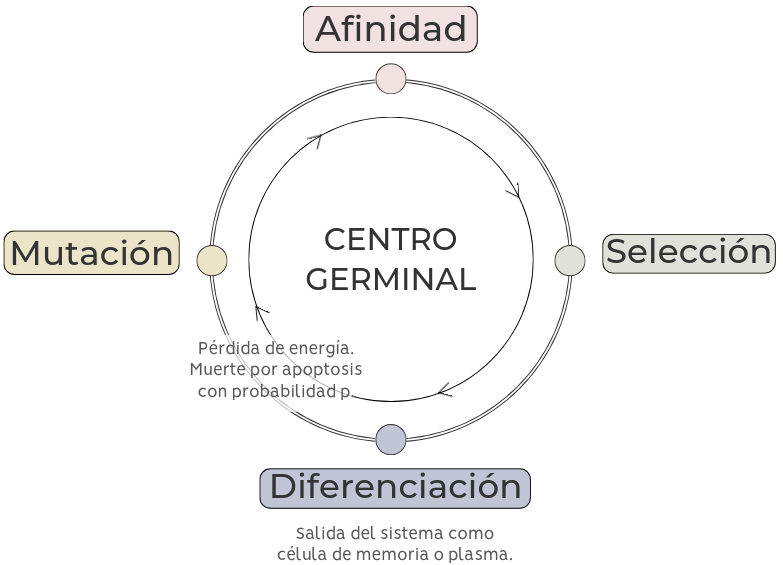
\includegraphics[width=1\textwidth]{Graphics/gc.png}
    \caption{Ciclo que ocurre dentro del Centro Germinal}
    \label{fig:cg}
\end{figure}

\section{Sistema Inmune}

El sistema inmune consta de un grupo de células B \textit{naive} que se dividen y mutan o mueren. Ante la presencia de antígeno estas células pueden pasar a formar parte de centros germinales como se muestra en la figura \ref{fig:is}. 

Al finalizar cada ciclo, los centros germinales liberan al sistema inmunológico células B diferenciadas en células plasmáticas y células de memoria. La concentración de anticuerpos generada por estas sirve como indicador cuantitativo de la respuesta inmunológica del individuo.

\begin{figure}[H] % h = here (aquí)
    \centering
    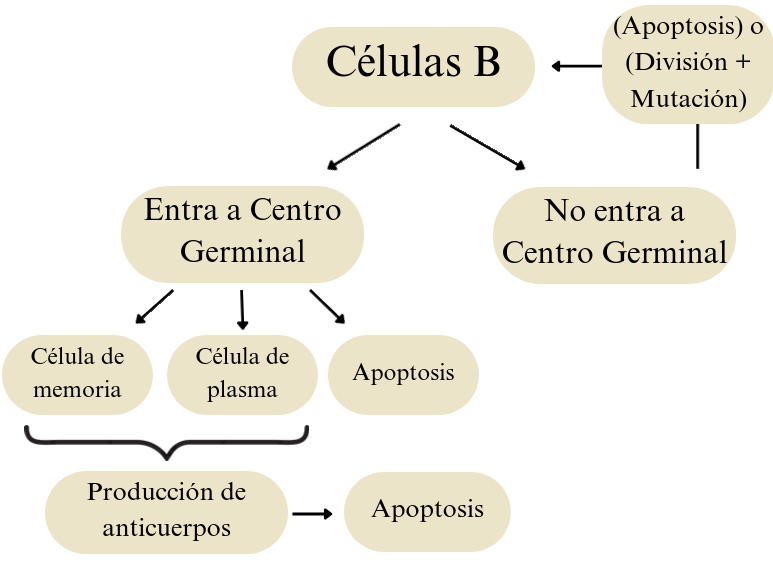
\includegraphics[width=1\textwidth]{Graphics/is.png}
    \caption{Células B dentro del sistema inmune}
    \label{fig:is}
\end{figure}




% aaaaaaaaaaaaaaaaaaaaaaaaaaaaaaaaaaaaaaaaaaaaaaaaaaaaaaaaaaaaaaaaaaaaaaaaaaaaaaaaaaa
% aaaaaaaaaaaaaaaaaaaaaaaaaaaaaaaaaaaaaaaaaaaaaaaaaaaaaaaaaaaaaaaaaaaaaaaaaaaaaaaaaaa
% aaaaaaaaaaaaaaaaaaaaaaaaaaaaaaaaaaaaaaaaaaaaaaaaaaaaaaaaaaaaaaaaaaaaaaaaaaaaaaaaaaa
% aaaaaaaaaaaaaaaaaaaaaaaaaaaaaaaaaaaaaaaaaaaaaaaaaaaaaaaaaaaaaaaaaaaaaaaaaaaaaaaaaaa
% aaaaaaaaaaaaaaaaaaaaaaaaaaaaaaaaaaaaaaaaaaaaaaaaaaaaaaaaaaaaaaaaaaaaaaaaaaaaaaaaaaa




%===================================================================================
% Chapter: Metodologia
%===================================================================================
\chapter{Resultados}\label{chapter:resultados}
%\addcontentsline{toc}{chapter}{Marco Teórico}
%===================================================================================

En este capítulo se detalla el proceso de validación del modelo propuesto. 

\section{Datos para la Validación del Modelo}
Los datos utilizados en la investigación provienen del Estudio en Lactantes Fase I/II para PCV7-TT (Instituto Finlay de Vacunas, 2019), cuyo principal objetivo era caracterizar la seguridad del candidato vacunal VCN7-T y evaluar la no inferioridad de VCN7-T con respecto a la vacuna Prevnar13® administrados en esquemas concomitante con las vacunas Va-Mengoc- BC® y Heberpenta® incluyendo lactantes de 2 a 3 meses de edad.

Se cuenta con datos de 240 sujetos divididos en dos grupos:
\begin{enumerate}
    \item Vacunados con VCN7-T
    \item Vacunados con Prevnar13®
\end{enumerate}

Para la validación del modelo nos centraremos en el grupo de sujetos vacunados con VCN7-T

\subsection{Limpieza de Datos}
Antes de trabajar con los datos fue realizado un proceso de limpieza de los mismos. 


\subsubsection{Análisis de Datos Faltantes}

Las Figuras \ref{fig:mdq} y \ref{fig:mdp} presentan el análisis de valores faltantes (nulos o vacíos) en las columnas de los conjuntos de datos para las vacunas VCN7-T (Figura \ref{fig:mdq}) y Prevnar13 (Figura \ref{fig:mdp}). 

\textbf{Descripción de las gráficas:}
\begin{itemize}
    \item \textbf{Eje Y:} Nombre de las columnas/variables del estudio
    \item \textbf{Eje X:} Cantidad de valores faltantes (expresada en conteo absoluto)
\end{itemize}

\begin{figure}[H]
    \centering
    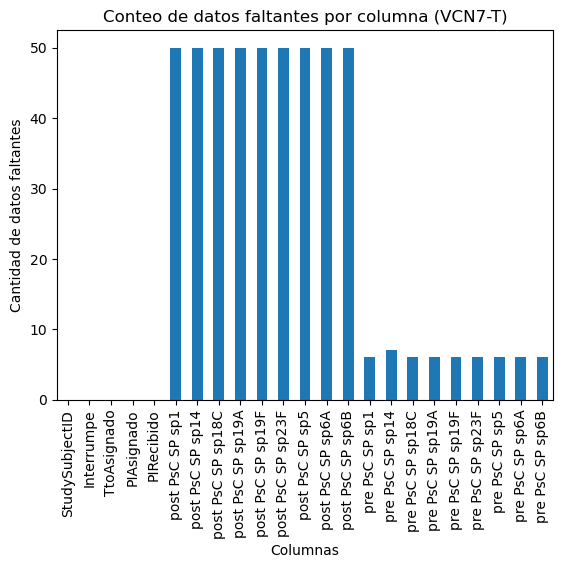
\includegraphics[width=0.7\textwidth]{Graphics/mdq.png}
    \caption{Distribución de valores faltantes por columna (VCN7-T)}
    \label{fig:mdq}
\end{figure}

\begin{figure}[H]
    \centering
    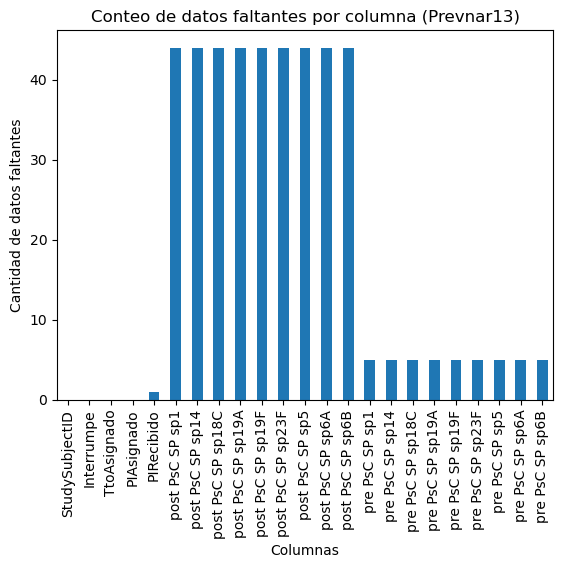
\includegraphics[width=0.7\textwidth]{Graphics/mdp.png}
    \caption{Distribución de valores faltantes por columna (Prevnar13)}
    \label{fig:mdp}
\end{figure}

La nomenclatura utilizada en los nombres de columna sigue este patrón:
\begin{itemize}
    \item \texttt{pre PsC SP [serotipo]:} Concentración de anticuerpos antes de la aplicación de la dosis de refuerzo (después de la dosis primaria) para un serotipo neumocócico específico
    \item \texttt{post PsC SP [serotipo]:} Concentración de anticuerpos después de la aplicación de la dosis de refuerzo para un serotipo neumocócico específico
    \item \texttt{[serotipo]:} Identificador del serotipo (e.g., sp1, sp14, sp19F, etc.)
\end{itemize}


Los altos valores en las columnas \texttt{post PsC SP [serotipo]} se consideran \textbf{no aleatorios} (MNAR - Missing Not At Random) y están directamente relacionados con el diseño del estudio, que incluyó dos esquemas de vacunación:

\begin{itemize}
    \item \textbf{Esquema (2p + 1):} Dos dosis primarias + refuerzo (mediciones post-refuerzo disponibles)
    \item \textbf{Esquema (3p + 0):} Tres dosis primarias sin refuerzo (mediciones post-refuerzo ausentes)
\end{itemize}

% Para la validación del modelo, se trabajó exclusivamente con los sujetos vacunados bajo el esquema (2p + 1), ya que:
% \begin{enumerate}
%     \item Presentan mediciones completas de anticuerpos post-vacunación
%     \item Permiten evaluar la respuesta inmune tras la dosis de refuerzo
%     \item Constituyen la cohorte con seguimiento completo
% \end{enumerate}

% \textbf{Justificación del enfoque:}
% La exclusión de sujetos con esquema (3p + 0) se basa en:
% \begin{itemize}
%     \item La imposibilidad de calcular la respuesta inmune completa sin mediciones post-vacunación
%     \item La necesidad de homogeneidad en el análisis de respuesta vacunal
%     \item La preservación de la validez interna del estudio
% \end{itemize}

En la investigación se asume que los sujetos con valores nulos en las columnas \texttt{post PsC SP [serotipo]} fueron vacunados siguiendo un esquema (3p + 0), sin embargo para la validación del modelo se trabajó en los sujetos vacunados siguiendo el esquema (2p + 1).

\subsubsection{Valores inconsistentes}
Durante el análisis de los datos, se detectaron valores atípicos con magnitudes aparentemente inconsistentes. Una inspección minuciosa reveló que dichos valores correspondían a cifras significativas expresadas con distinta notación decimal; en particular, mientras la mayoría de los datos estaban representados con tres cifras significativas correctamente posicionadas, algunos carecían del punto decimal, lo que implicaba una escala incorrecta. Para homogeneizar la representación, se aplicó una corrección que consiste en dividir por 1000 los valores afectados. Esta normalización facilitó una presentación más coherente y uniforme de los datos.

En las gráficas \ref{fig:sp1d}, \ref{fig:sp1}, \ref{fig:sp14d} y \ref{fig:sp14} (Gráficas de valores pre-refuerzo contra valores post-refuerzo) se muestra una comparación del estado de los datos antes y después de la corrección (las gráficas para el resto de los serotipos se muestran en \ref{comp}). 


\begin{figure}[h]
    \centering
    % Primera fila
    \begin{minipage}{0.45\textwidth}
        \centering
        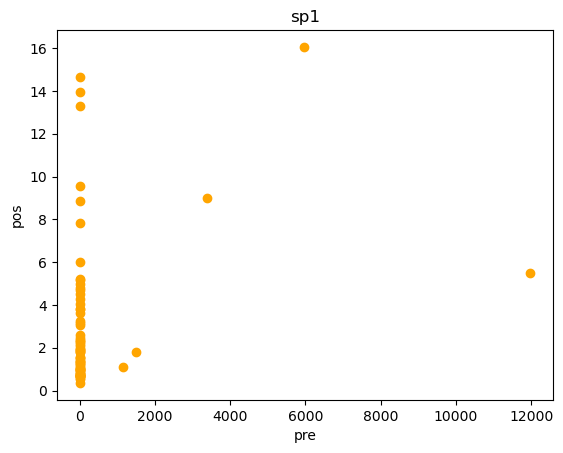
\includegraphics[width=\linewidth]{Graphics/sp1d.png}
        \caption{Serotipo 1 antes de la corrección}
        \label{fig:sp1d}
    \end{minipage}%
    \hfill
    \begin{minipage}{0.45\textwidth}
        \centering
        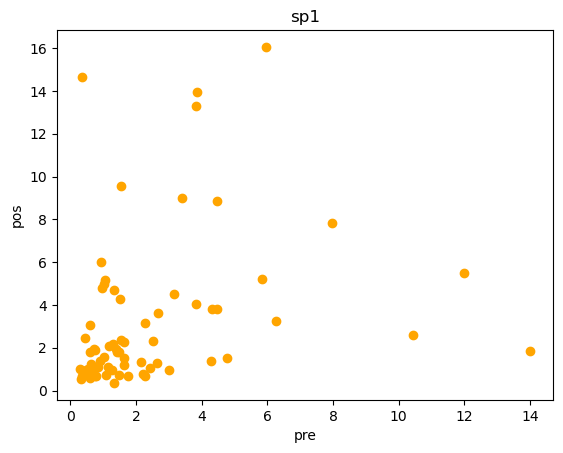
\includegraphics[width=\linewidth]{Graphics/sp1.png}
        \caption{Serotipo 1 después de la corrección}
        \label{fig:sp1}
    \end{minipage}

\end{figure}

\begin{figure}[H]
    \begin{minipage}{0.45\textwidth}
        \centering
        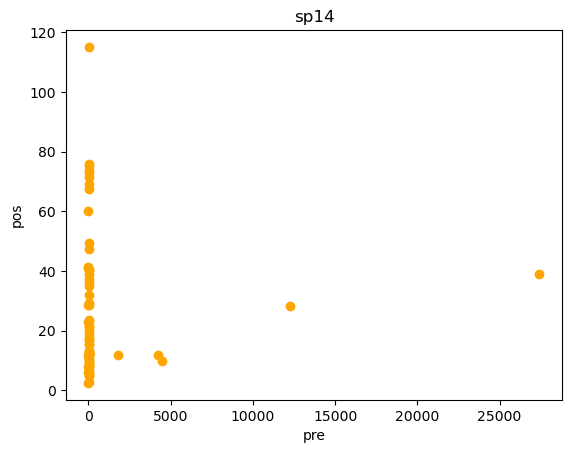
\includegraphics[width=\linewidth]{Graphics/sp14d.png}
        \caption{Serotipo 14 antes de la corrección}
        \label{fig:sp14d}
    \end{minipage}%
    \hfill
    \begin{minipage}{0.45\textwidth}
        \centering
        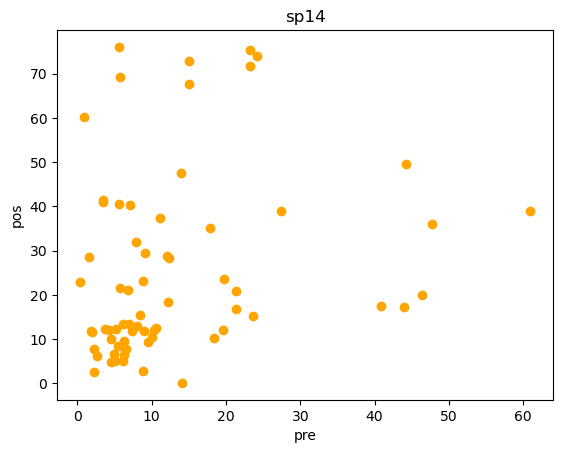
\includegraphics[width=\linewidth]{Graphics/sp14.png}
        \caption{Serotipo 14 después de la corrección}
        \label{fig:sp14}
    \end{minipage}
\end{figure}

En las gráficas pre-procesamiento de observan datos en el orden de las decenas de miles en el eje de las X los cuales pueden ser considerados como \textit{outliers} por un análisis superficial. Sin embargo después de aplicada la corrección antes expuesta estos puntos responden más adecuadamente a la naturaleza de los datos.


\section{Entrenamiento}
Para el entrenamiento del modelo se tomó el 70\% de los datos. Este proceso tiene como objetivo estimar los parámetros \texttt{plasma\_production\_factor} y \texttt{memory\_production\_factor}.

\subsection{Exploración del espacio de parámetros}

Para explorar el espacio de parámetros durante el proceso de entrenamiento se utilizó la metaheurística de Recocido Simulado (\textit{Simulated Annealing}). Este método permitió realizar una búsqueda estocástica evitando quedar atrapado en óptimos locales, gracias a su capacidad para aceptar temporalmente soluciones peores con una probabilidad controlada por un parámetro denominado temperatura.

El algoritmo comienza con una temperatura inicial 1.0 que permite explorar el espacio de soluciones, aceptando cambios incluso si empeoran la función objetivo. A medida que avanza el proceso, la temperatura decrece siguiendo un protocolo de enfriamiento, reduciendo gradualmente la probabilidad de aceptar soluciones peores.

\subsubsection{Soluciones vecinas:}
Estas se generan seleccionando aleatoriamente uno de los parámetros a estimar y añadiéndole un ajuste $\delta$.

\subsubsection{Criteros de parada:}
\begin{itemize}
    \item \textbf{Enfriamiento del metal:} la temperatura es menor que \texttt{1e-3}.
    \item \textbf{Máximo de iteraciones:} se realizan más de 100 iteraciones.
\end{itemize}



\subsection{Función Objetivo}

La métrica utilizada como función objetivo durante el entrenamiento del modelo es la \textit{distancia de Chamfer} ($D_{\mathrm{Chamfer}}(S_1, S_2)$, donde \( S_1 \) y \( S_2 \) son los conjuntos de puntos simulados y reales), que es adecuada para comparar nubes de puntos, ya que evalúa la proximidad bidireccional entre cada punto de un conjunto y su vecino más cercano en el otro conjunto.

Minimizar la distancia de Chamfer durante el entrenamiento guía al modelo a generar salidas que se ajusten a los datos.


\section{Validación}
Para el proceso de validación se tomó el 30\% restante de los datos. Se generó una conjunto de la misma cantidad de puntos con los parámetros obtenidos en el proceso de entrenamiento y se calculó la distancia Chamfer para estos conjuntos. Los resultados obtenidos se muestran en la tabla \ref{tab:chamfer_serotipos}:

\begin{table}[h]
\centering
\caption{Distancia de Chamfer por Serotipo}
\begin{tabular}{|c|c|}
\hline
\textbf{Serotipo} & \textbf{Distancia Chamfer} \\
\hline
1   & 3.422  \\
14  & 26.348 \\
18C & 2.773  \\
19F & 4.443  \\
23F & 4.803  \\
5   & 3.241  \\
6B  & 8.539  \\
\hline
\end{tabular}
\label{tab:chamfer_serotipos}
\end{table}
Aunque los resultados visuales y cuantitativos no son óptimos, aportan información valiosa a la investigación. El modelo presenta un menor desempeño en serotipos, como el 14 y el 6B, cuyos datos experimentales exhiben una mayor dispersión (nube de puntos más amplia), lo que sugiere que su precisión podría mejorar con un tamaño de muestra más grande.

En las gráficas, desde la \ref{fig:sp1t} hasta la \ref{fig:sp6bt}, se observa que, si bien la salida del modelo no captura por completo la variabilidad de los datos, logra aproximarse al centroide de la distribución. Esta aproximación es más precisa en los serotipos donde la dispersión de los datos es menor.

El 

\textbf{Gráficas de valores pre-refuerzo (post vacunación primaria) contra valores post-refuerzo}
\begin{itemize}
    \item Puntos naranjas: datos de validación.
    \item Puntos azules: salida del modelo.
    \item Punto violeta: centroide de los datos de validación.
\end{itemize}
\begin{figure}[h]
    \centering
    % Primera fila
    \begin{minipage}{0.45\textwidth}
        \centering
        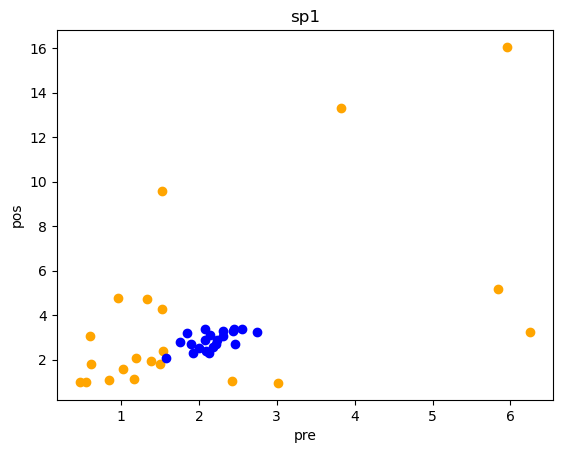
\includegraphics[width=\linewidth]{Graphics/sp1t.png}
        \caption{Serotipo 1}
        \label{fig:sp1t}
    \end{minipage}%
    \hfill
    \begin{minipage}{0.45\textwidth}
        \centering
        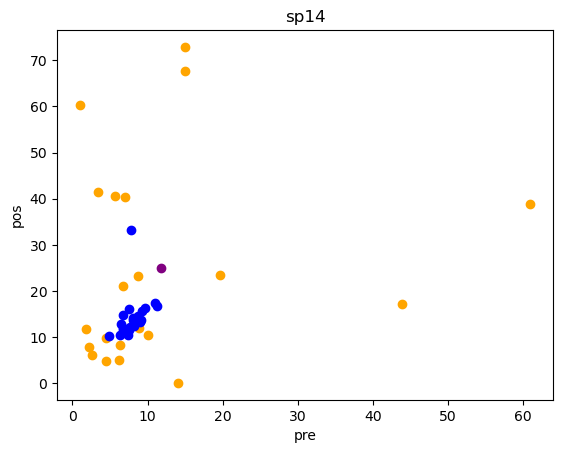
\includegraphics[width=\linewidth]{Graphics/sp14t.png}
        \caption{Serotipo 14}
        \label{fig:sp14t}
    \end{minipage}
\end{figure}
\begin{figure}
    
    \begin{minipage}{0.45\textwidth}
        \centering
        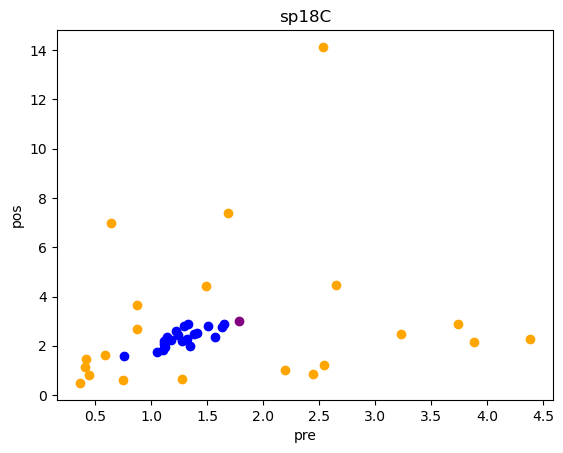
\includegraphics[width=\linewidth]{Graphics/sp18ct.png}
        \caption{Serotipo 18C}
        \label{fig:sp18ct}
    \end{minipage}
    \begin{minipage}{0.45\textwidth}
        \centering
        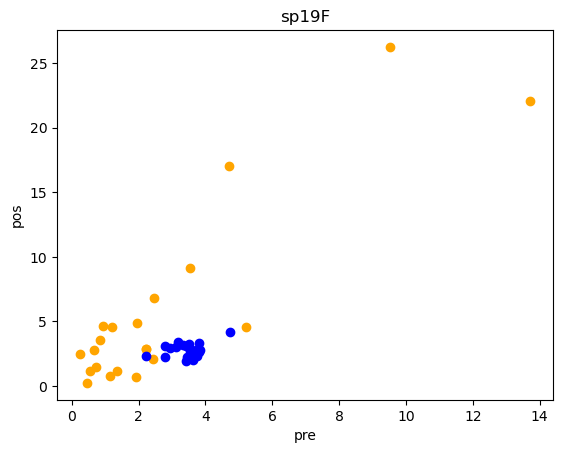
\includegraphics[width=\linewidth]{Graphics/sp19ft.png}
        \caption{Serotipo 19F}
        \label{fig:sp19ft}
    \end{minipage}
\end{figure}
\begin{figure}
    \begin{minipage}{0.45\textwidth}
        \centering
        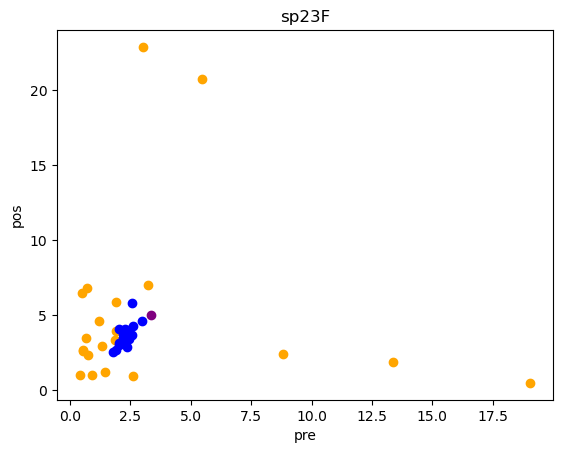
\includegraphics[width=\linewidth]{Graphics/sp23ft.png}
        \caption{Serotipo 23F}
        \label{fig:sp23ft}
    \end{minipage}
    \begin{minipage}{0.45\textwidth}
        \centering
        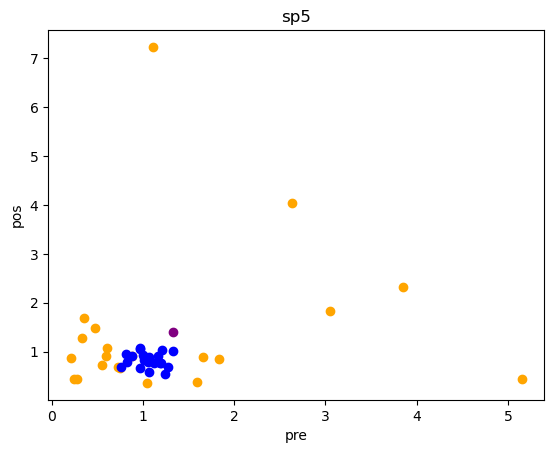
\includegraphics[width=\linewidth]{Graphics/sp5t.png}
        \caption{Serotipo 5}
        \label{fig:sp5t}
    \end{minipage}
\end{figure}
\begin{figure}
    \begin{minipage}{0.45\textwidth}
        \centering
        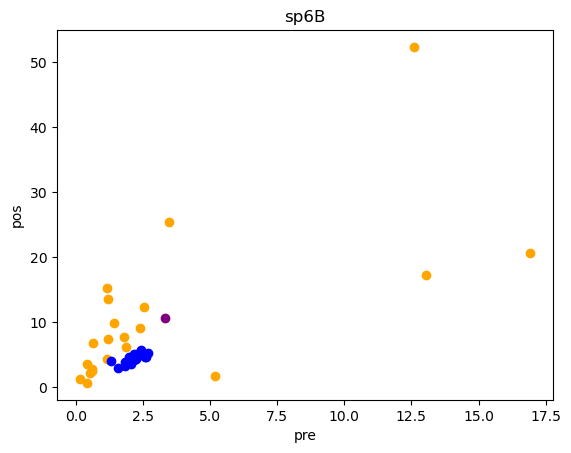
\includegraphics[width=\linewidth]{Graphics/sp6bt.png}
        \caption{Serotipo 6B}
        \label{fig:sp6bt}
    \end{minipage}

\end{figure}



%\backmatter
%===================================================================================
% Chapter: Conclusiones
%===================================================================================
\chapter*{Conclusiones}\label{chapter:conclusions}
\addcontentsline{toc}{chapter}{Conclusiones}

Pending...


%===================================================================================
% Chapter: Conclusiones
%===================================================================================
\chapter*{Recomendaciones}\label{chapter:recomendations}
\addcontentsline{toc}{chapter}{Recomendaciones}

\begin{itemize}
    \item Dar continuidad al desarrollo del simulador utilizando los resultados una vez realizado el ensayo clínico para el candidato vacunal futuro, QuimiVio-11 (que incluye 4 nuevos serotipos). Esto permitirá fortalecer la confiabilidad predictiva del modelo mediante una validación empírica más amplia.

    \item Implementar técnicas de optimización para abordar posibles casos de subajuste, especialmente en serotipos con mayores distancias de Chamfer (ej. serotipo 14). 
    % Esto podría incluir la ampliación la exploración del espacio de parámetros


    \item Añadir complejidad al modelo mejorando la fidelidad biológica del modelo integrando elementos clave de la inmunidad innata como receptores de reconocimiento de patrones o dinámica de células fagocíticas (neutrófilos, macrófagos).
    

    \item Adaptar el simulador para modelar respuestas inmunes en diferentes poblaciones, especialmente para el adulto mayor, mediante el desarrollo de conjuntos de parámetros específicos por edad y la consideración de inmunosenescencia en población geriátrica.
    
    \item Tener en cuenta para la realización de próximos ensayos clínicos la posibilidad de realizar más de un examen de sangre a los pacientes en diferente cantidad de días post-vacunación.

\end{itemize}
\renewcommand{\bibname}{Referencias}
% \nocite{*}
\bibliographystyle{unsrt}
\bibliography{Bibliography.bib}
%\include{BackMatter/References}
%\include{BackMatter/Glossary}


\end{document}